%! TeX program = lualatex
%---------------------------ALLGEMEINE IMPORTS-------------------------------------
\documentclass[12pt,english,ngerman]{scrartcl}
\input{./protokoll_template/template.latex/input/shared_preamble.tex}

% Kopfzeile
\ihead{WS22\\
	21.12.2022} \chead{\textsc{Stark} Matthias - 12004907 \\
	\textsc{Philipp} Maximilian - 11839611}
\ohead{FLAB 1 \\
	Rasterelektronenmikroskopie}
% Fußzeile


\begin{document}

\section{Grundlagen}

%(max. 1 Seite)


\section{Proben- und Geräteliste}


\section{Kennenlernen des REM}


Zunächst wird die Probe mit einer Pinzette vorsichtig auf den Probentisch platziert. Für ein effektives Arbeiten können 
mehrere Proben gleichzeitig auf die Probenbühne gesetzt und diese zwischen den einzelnen Messungen einfach weitergedreht
werden. Im Rahmen des Praktikums wird jedoch immer nur eine Probe eingelegt, um das Handling zu lernen und sicherzustellen,
dass die "z-Ebene", also die Höhe, immer richtig eingestellt ist. Die Orientierung in dei "z-Achse" wird fixiert, um 
sicherzustellen, dass kein "crash" verursacht wird.

Bei der Probe ist zu beachten, dass diese elektrisch leitfähig sein muss. Ist die Probe von sich aus schon leitfähig, wird
sie mit einem speziellen, leitenden Kohlenstoff-Band am Sockel befestigt. Handelt es sich um eine nicht leitende Probe, so 
muss die leitfähigkeit z.B. durch eine Platin Bedampfung gewährleistet werden, wie im \autoref{fig:probe} sichtbar.

\begin{figure}[H]
	\begin{center}
		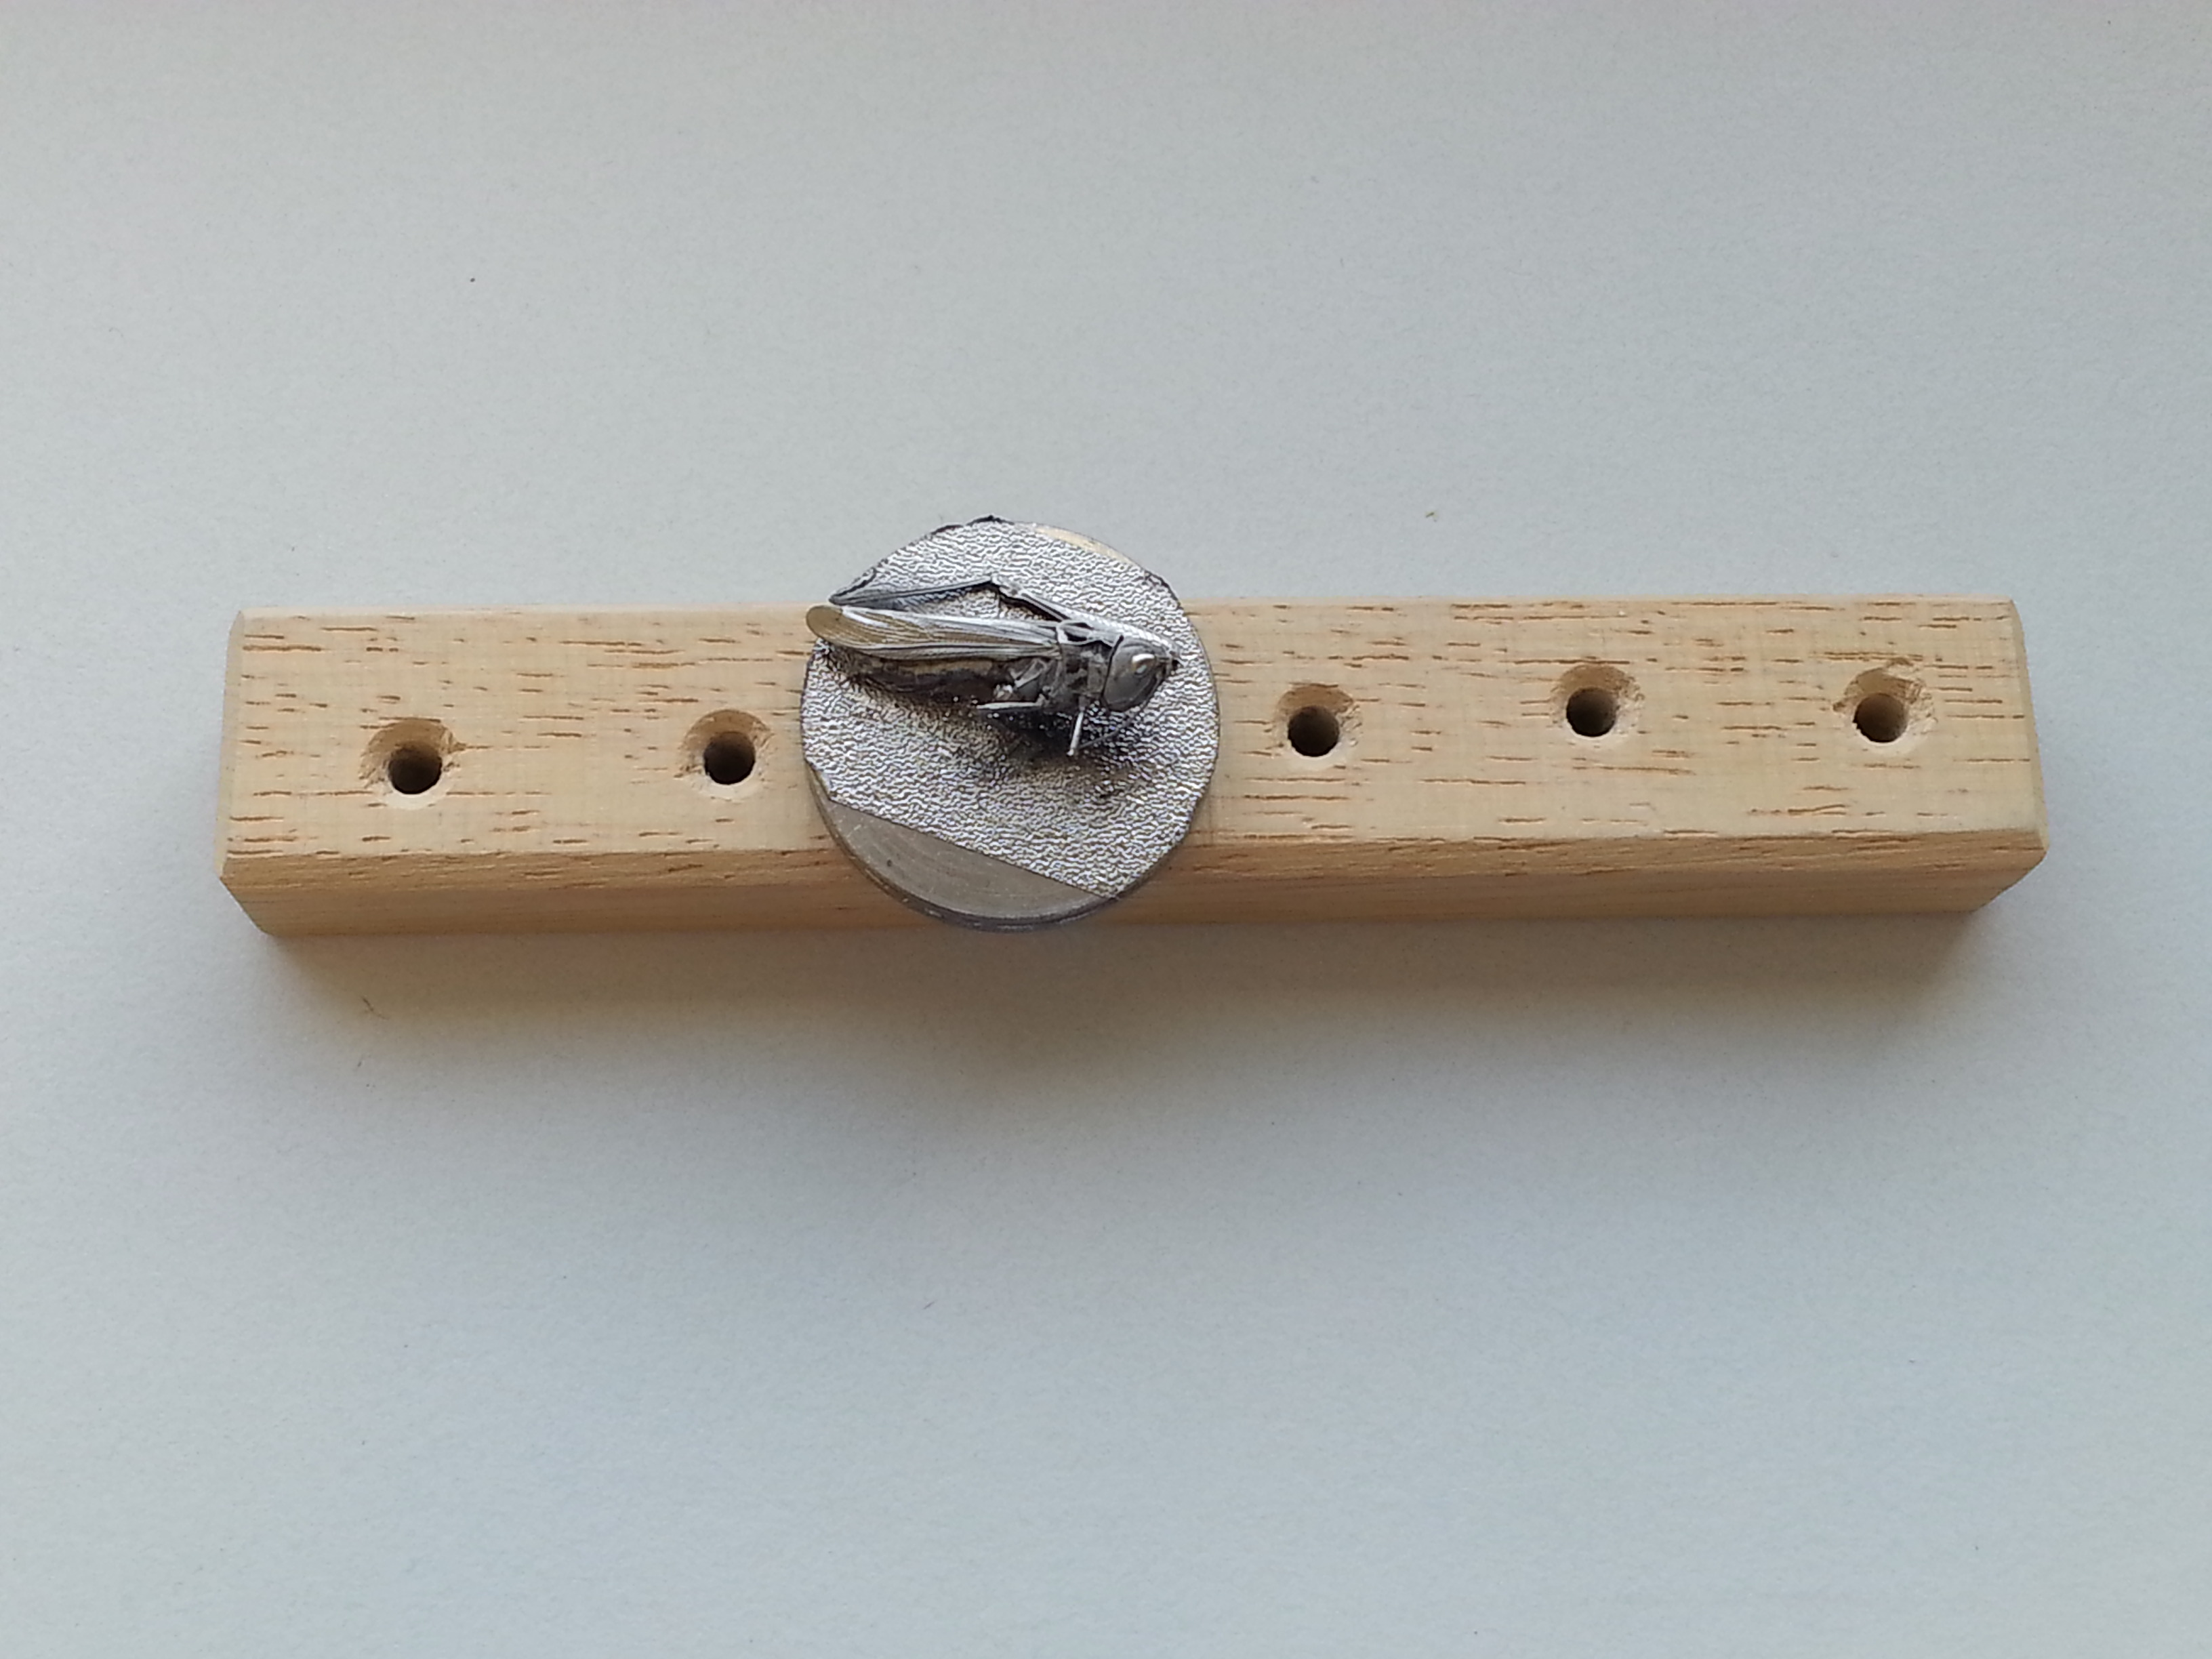
\includegraphics[width =0.5\textwidth]{./figures/probe.png}
	\end{center}
	\caption[Bedampfte, organische Probe]
	{Bedampfte, organische Probe \cite{sein_foto}}
    \label{fig:probe}
\end{figure}

Nach dem Einlegen der Probe wird ein Vakuum erzeugt, welches für den Betrieb des Elektronenmikroskops notwendig ist, was 
\SI{162(1)}{\s}, also keine \SI{3}{\min} dauert.

Nun wird das aufgezeichnete Bild im verwendeten Computerprogramm sichtbar. Durch Bewegung mit der Computermaus kann 
der entsprechende Bereich ausgewählt und die Vergrößerung eingestellt werden. Auch kann über den entsprechenden Knopf die 
Schärfe, sowie der Kontrast, variiert werden, um ein möglichst gut aufgelöstes Bild zu erreichen. Man muss sich bewusst 
sein, dass wie bei allen
optischen Aufbauten, gewisse Abbildungsfehler vorliegen. Für eine genauere Erklärung hierzu, sein auf \cite{unterlagen} 
verwiesen. Der Astigmatismus durch eine entsprechende Anpassung im jeweiligen Menüpunkt großteils behoben werden.


%todo gets vlt dass wir jeweils 2 Bilder nebeneinander kriegen? 

Im folgenden ist eine Auswahl der erzeugten Bilder angeführt. In \autoref{fig:auge} und \autoref{fig:auge2} sind Aufnahmen
des Facettenauges sichtbar. In \autoref{fig:flugel} sieht man die Struktur des Flügels und in \autoref{fig:damage} ist eine
komisch geformte Struktur sichtbar, die auf einen Fehler in der Bedampfungsschicht zurückzuführen ist.
Generell ist zu Beachten, dass der Elektronenstrahl nicht zu lange fokussiert auf eine bestimmte Stelle gerichtet wird, um
keinen "Beam-Damage" zu verursachen.

\begin{figure}[H]
	\begin{center}
		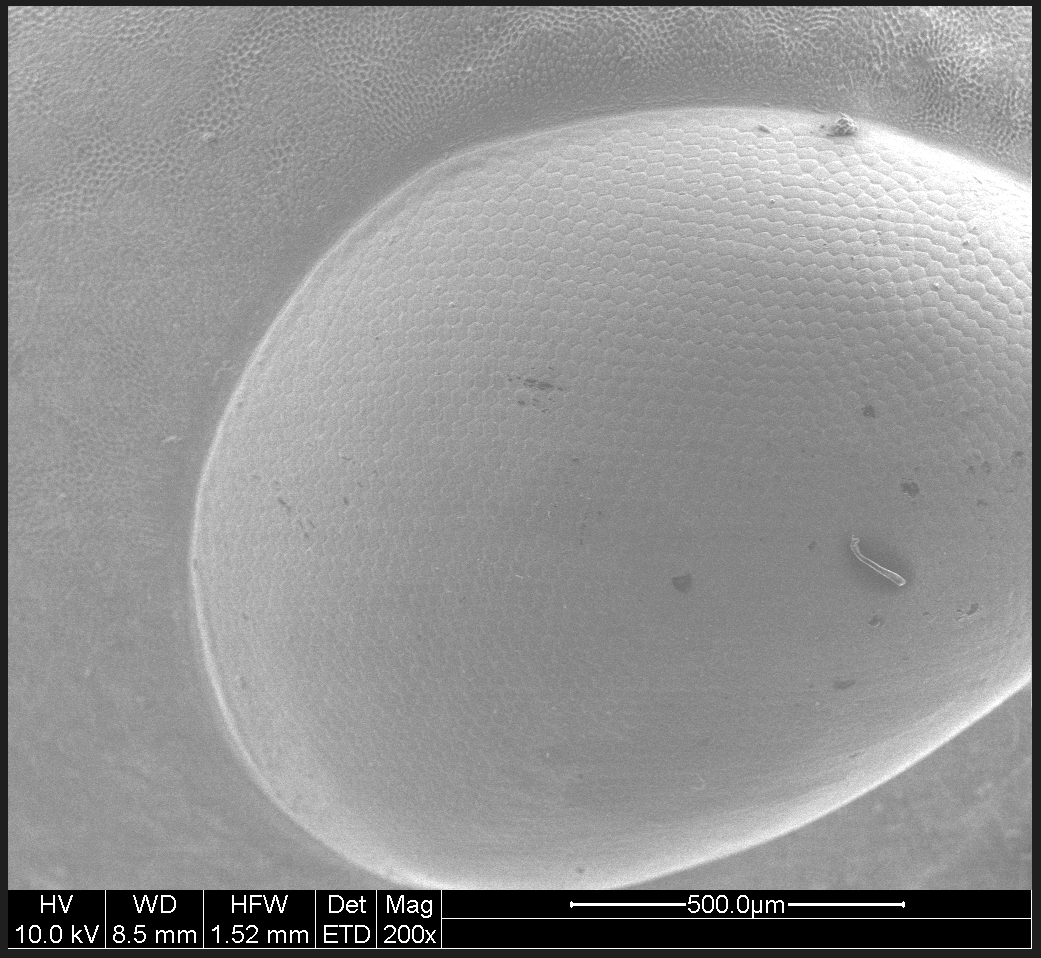
\includegraphics[width =0.5\textwidth]{./figures/auge.png}
	\end{center}
	\caption{Facettenauge}
    \label{fig:auge}
\end{figure}

\begin{figure}[H]
	\begin{center}
		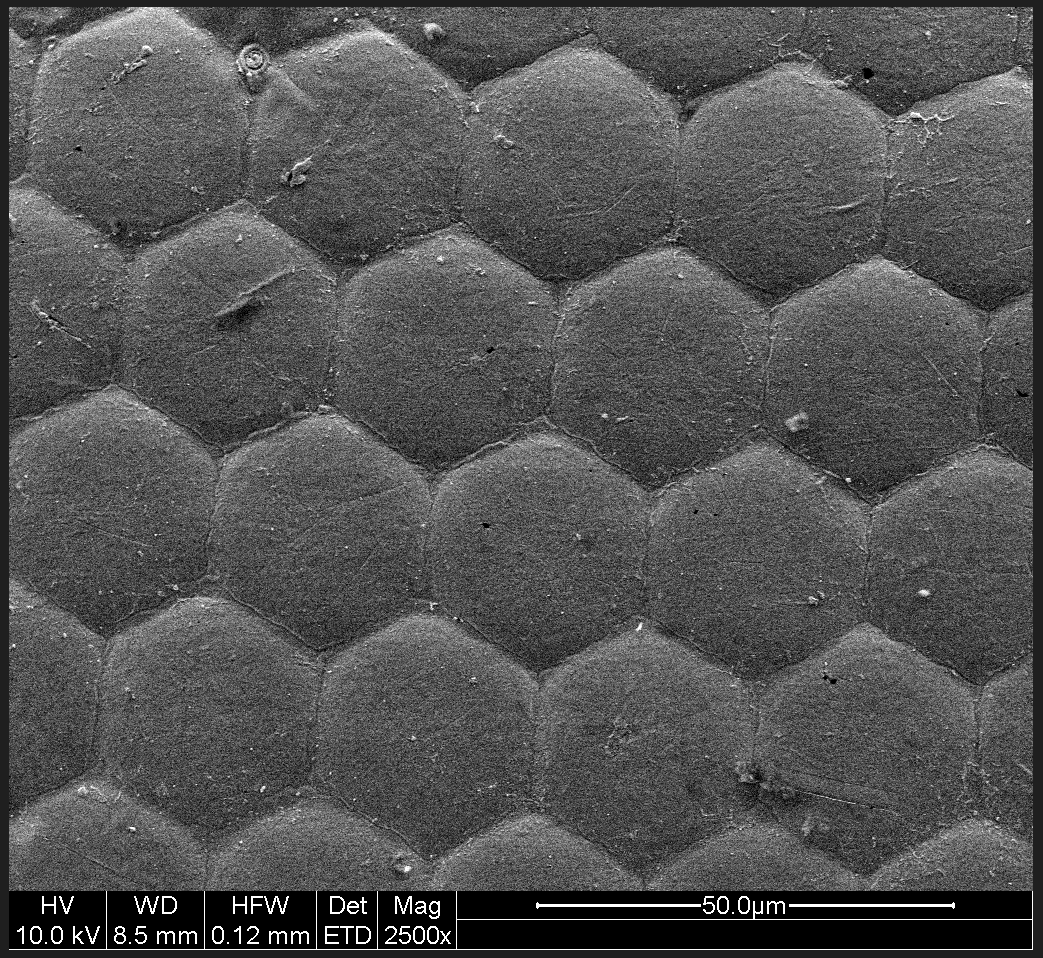
\includegraphics[width =0.5\textwidth]{./figures/auge2.png}
	\end{center}
	\caption{stärker vergrößertes Facettenauge}
    \label{fig:auge2}
\end{figure}

\begin{figure}[H]
	\begin{center}
		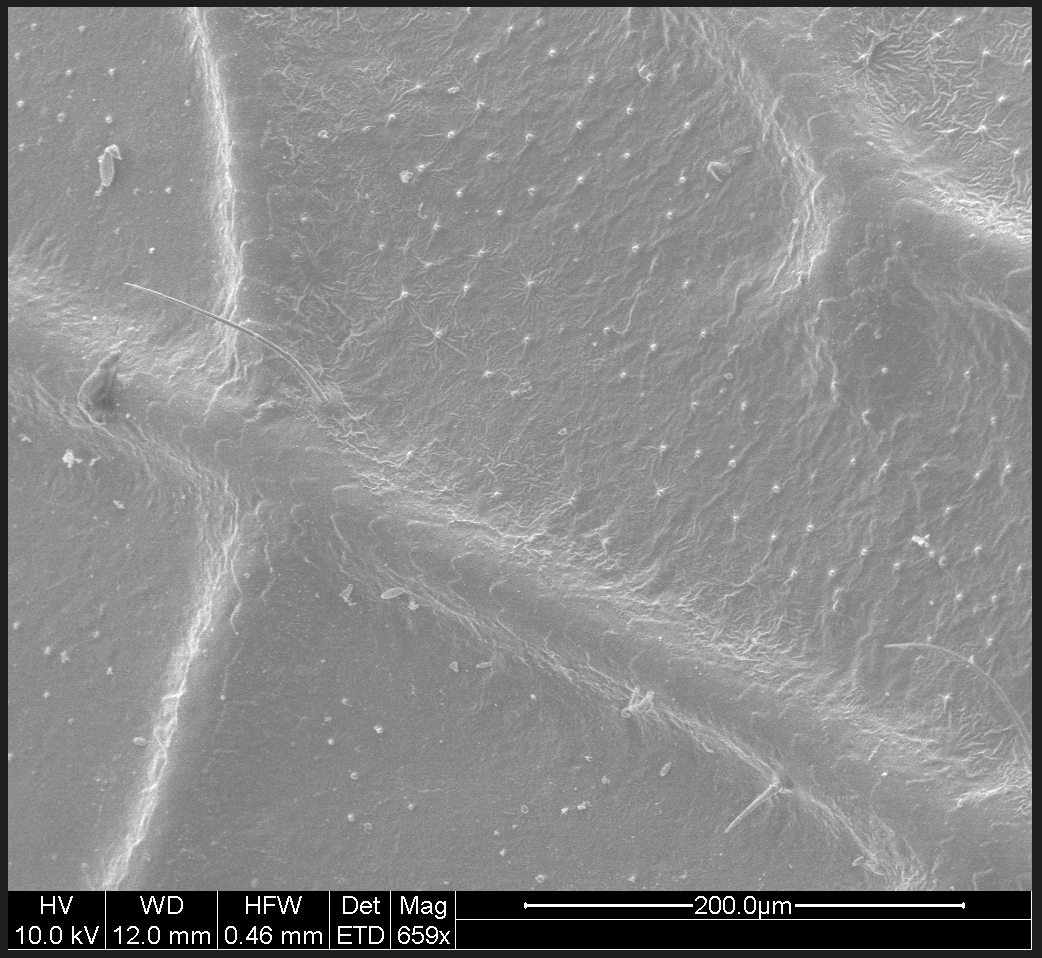
\includegraphics[width =0.5\textwidth]{./figures/flugel.png}
	\end{center}
	\caption{Struktur des Flügels}
    \label{fig:flugel}
\end{figure}

\begin{figure}[H]
	\begin{center}
		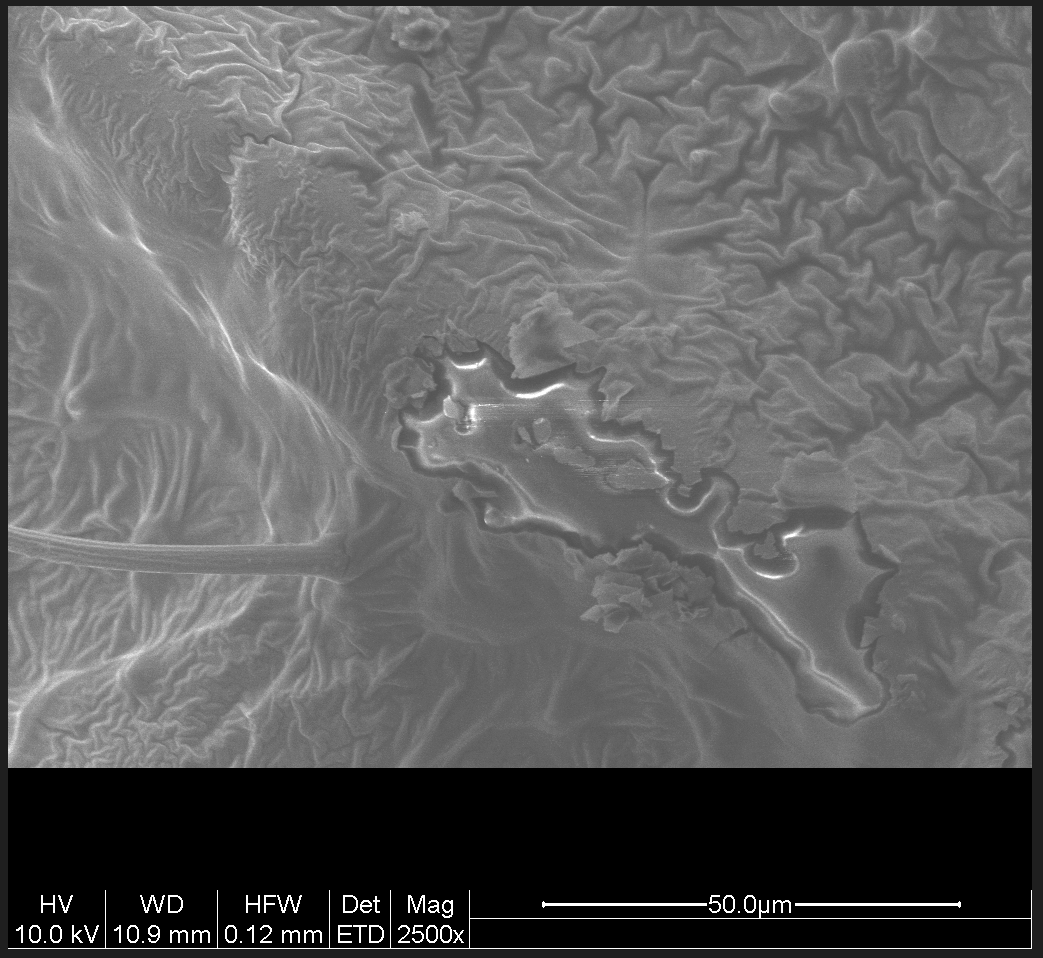
\includegraphics[width =0.5\textwidth]{./figures/damage.png}
	\end{center}
	\caption{Fehler in Bedampfungsschicht}
    \label{fig:damage}
\end{figure}


\section{Polypropylen-Gewebe}

Nun wird ein teilweise beschichtetes Stück eines Polypropylen Gewebes in den Aufbau gegeben, wie in \autoref{fig:aufbau} sichtbar.

\begin{figure}[H]
	\begin{center}
		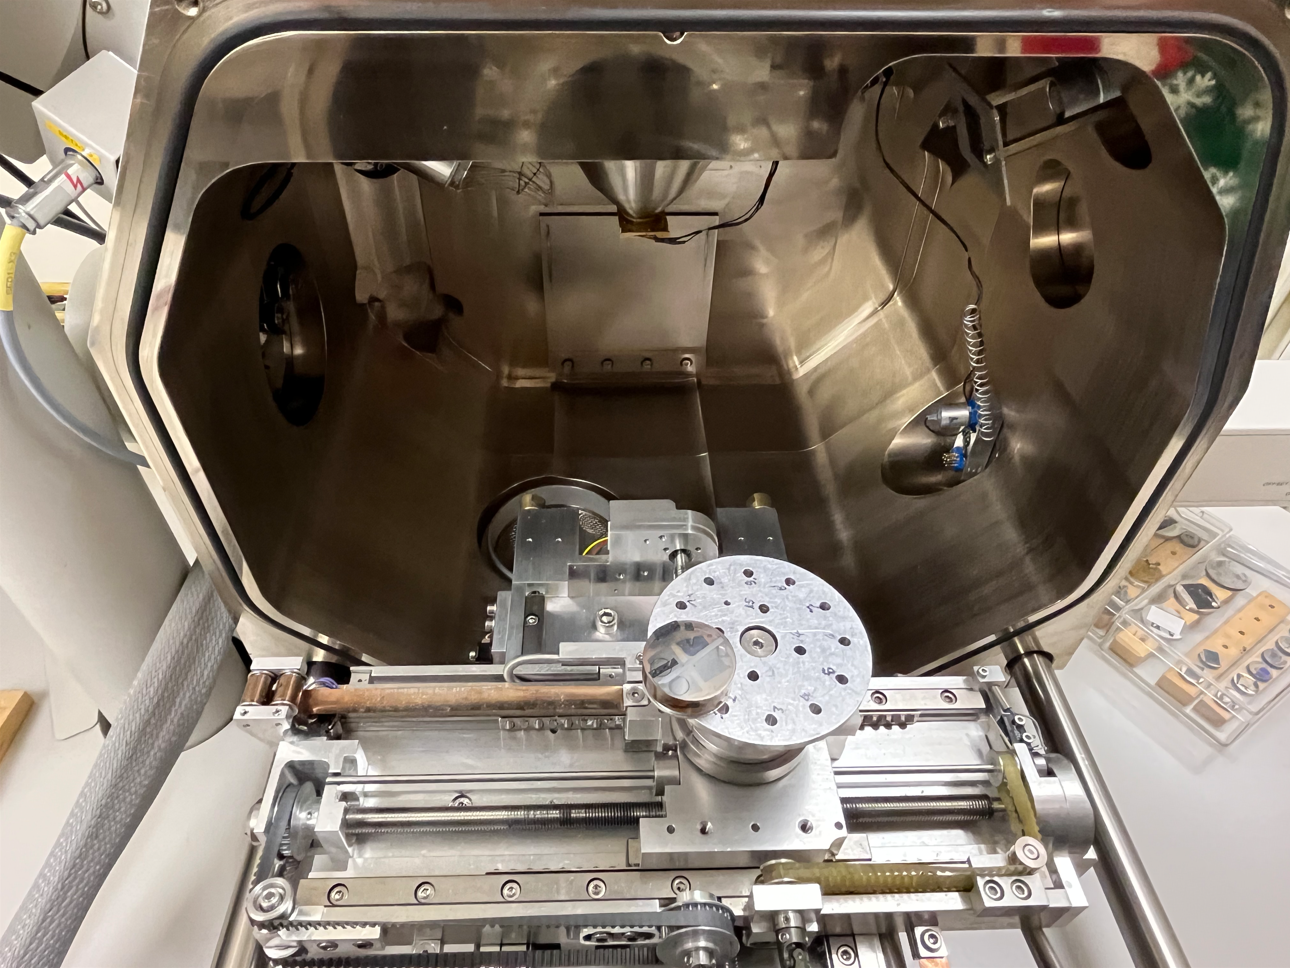
\includegraphics[width =0.5\textwidth]{./figures/aufbau.png}
	\end{center}
	\caption{Polypropylen Gewebe in Versuchsaufbau}
    \label{fig:aufbau}
\end{figure}


\subsection{Vergleich „beschichtet“ und „unbeschichtet“}

Zunächst dir jeweils eine Beschichtete und eine un beschichtete Position auf der Probe als Position markiert, um einen
unproblematischen Wechsel zwischen ihnen zu ermöglichen. Die Betrachtung der erzeugten Bilder zeigt sofort, dass im 
beschichteten Zustand viel schärfere Fotos erzeugt werden können, wie im nächsten Kapitel ersichtlich. Betrachtet man 
den unbeschichteten Zustand, wie in \autoref{fig:unbeschichtet} sichtbar, wird deutlich, dass am Präparat feine 
Bewegungen der Struktur sichtbar sind, was an den ruckartigen Unterbrechungen in folgender \autoref{fig:unbeschichtet}
sichtbar wird. Besonders leicht erkennbar werden diese Bewegungen, wenn mehrere Bilder aufgezeichnet werden und diese 
dann als Film abgespielt werden, was im Rahmen dieses Protokolls aber leider nicht geteilt werden kann.

\begin{figure}[H]
	\begin{center}
		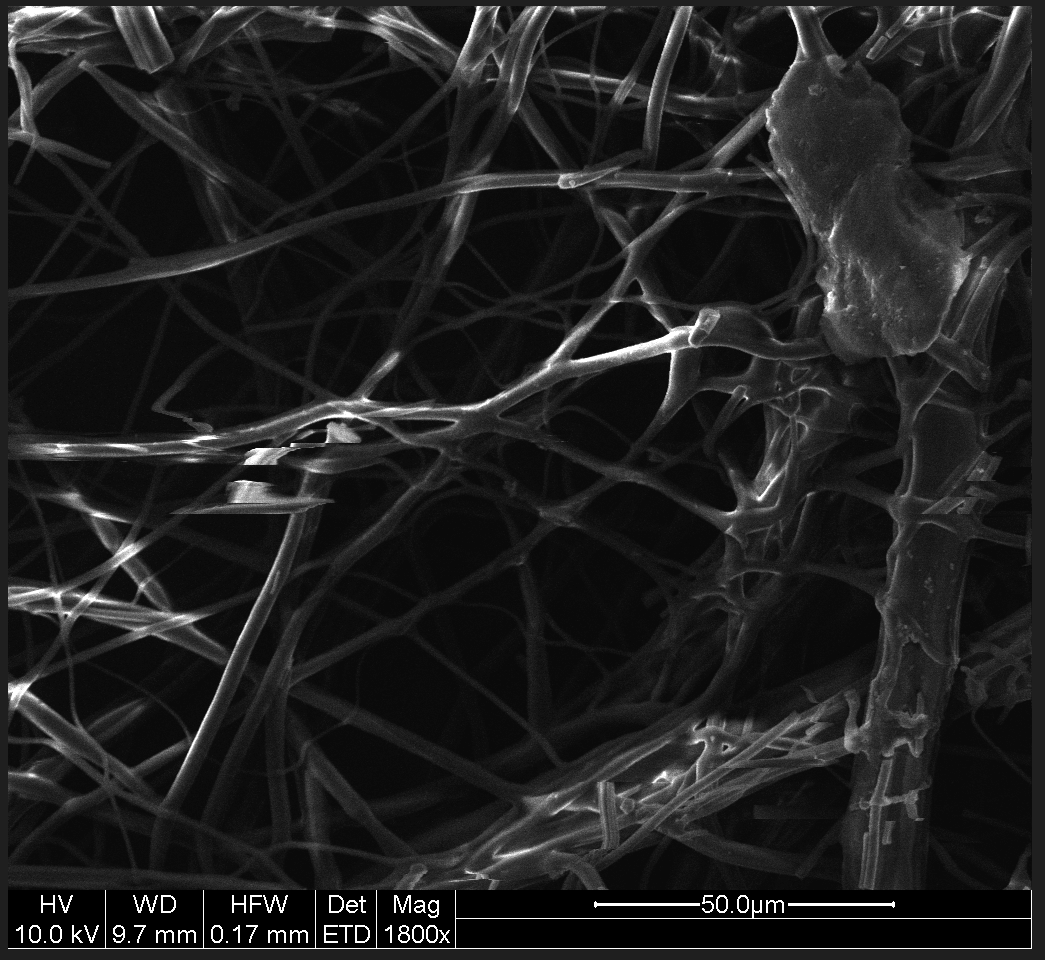
\includegraphics[width =0.5\textwidth]{./figures/unbedampft.png}
	\end{center}
	\caption{Unbeschichtetes Polypropylen Gewebe}
    \label{fig:unbeschichtet}
\end{figure}

\subsection{Variation der Beschleunigungsspannung}

In diesem Teil des Versuchs wird die Beschleunigungsspannung der Elektronen variiert. Wenn diese größer ist, können die 
Elektronen in tiefere SChichten der Probe eindringen, weshalb die oberen, dünnen Schichten transparent wirken. 

%todo max du hast die referenzen einmal zusammengefasst i finds aber nicht mehr
Die erzeugten Bilder sind in \autoref{{fig:5kv},{fig:10kv},{fig:20kv},{fig:30kv}} ersichtlich. 
Zusätzlich wurden Monte Carlo Simulationen zur Verfügung gestellt, die die Bewegung der Elektronen nach den Streuungen
darstellen, siehe \autoref{fig:simulation5kv},\autoref{fig:simulation10kv},\autoref{fig:simulation20kv},\autoref{fig:simulation30kv}.

%todo es wäre schön wenn auch hier immer Bild und simulation nebeneinander wären

\begin{figure}[H]
	\begin{center}
		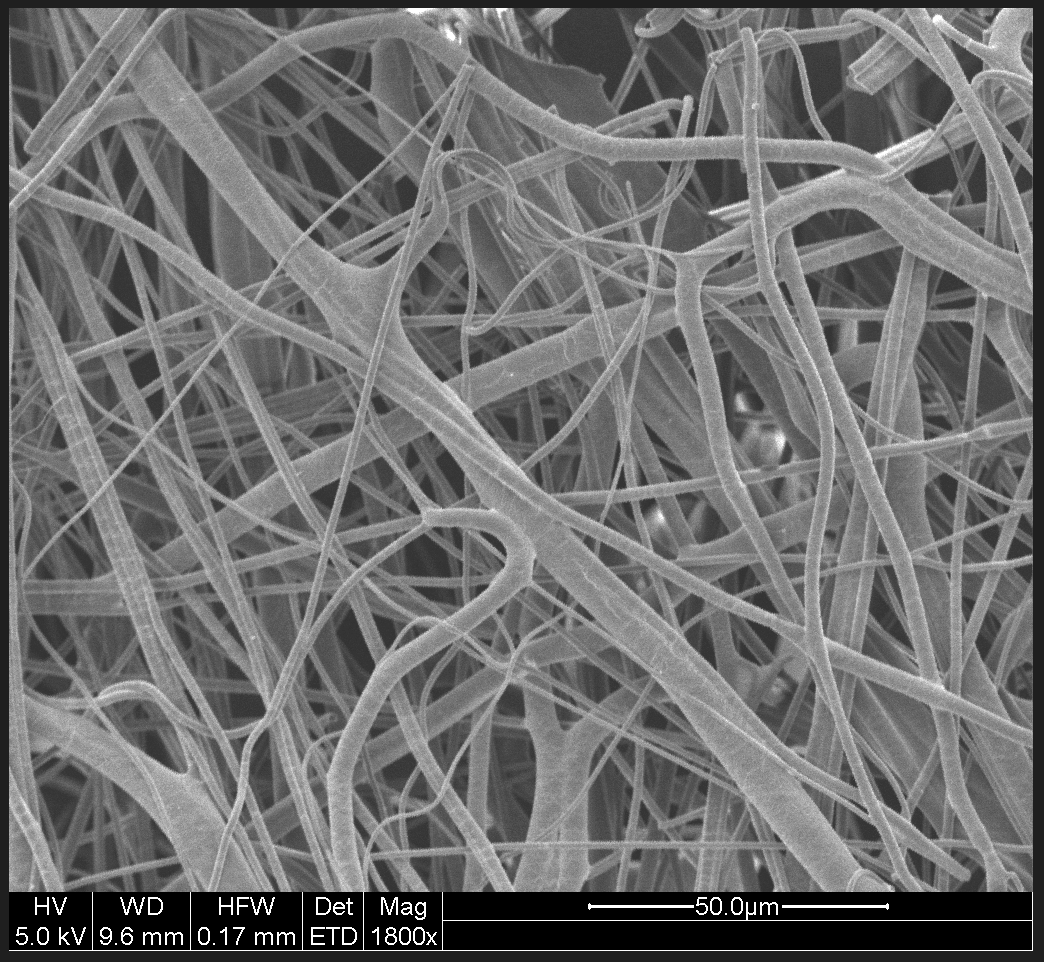
\includegraphics[width =0.5\textwidth]{./figures/5kv.png}
	\end{center}
	\caption{Sichtbares Bild bei einer Beschleunigungsspannung von \SI{5}{\kilo\volt}}
    \label{fig:5kv}
\end{figure}

\begin{figure}[H]
	\begin{center}
		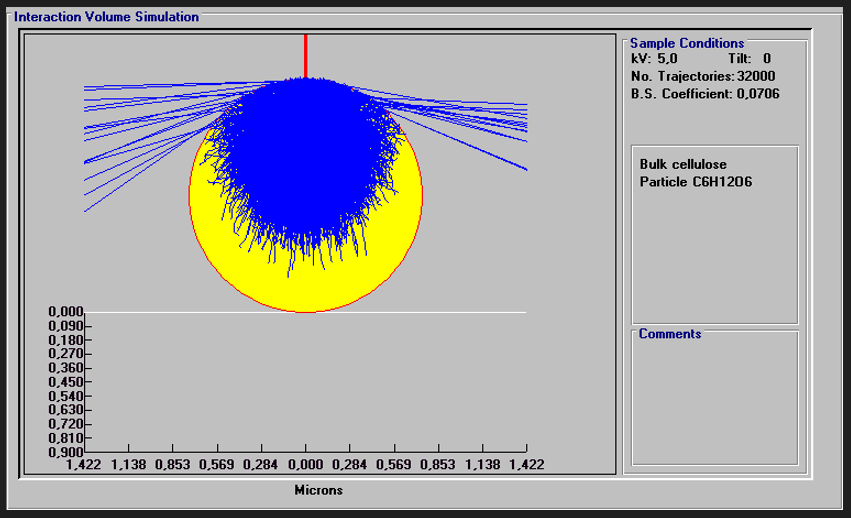
\includegraphics[width =0.5\textwidth]{./figures/simulation5kv.png}
	\end{center}
	\caption{Erzeugte Simulation bei einer Beschleunigungsspannung von \SI{5}{\kilo\volt}}
    \label{fig:simulation5kv}
\end{figure}


\begin{figure}[H]
	\begin{center}
		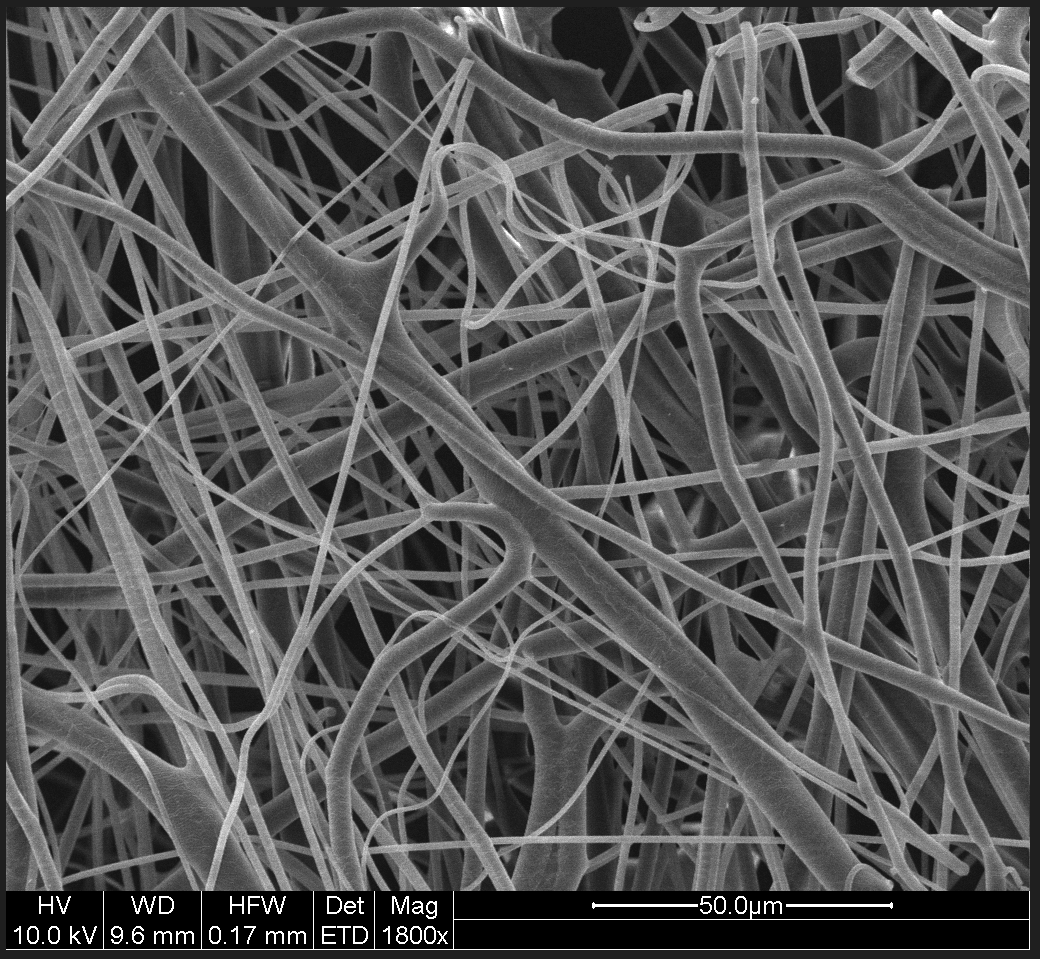
\includegraphics[width =0.5\textwidth]{./figures/10kv.png}
	\end{center}
	\caption{Sichtbares Bild bei einer Beschleunigungsspannung von \SI{10}{\kilo\volt} \cite{sein_foto}}
    \label{fig:10kv}
\end{figure}

\begin{figure}[H]
	\begin{center}
		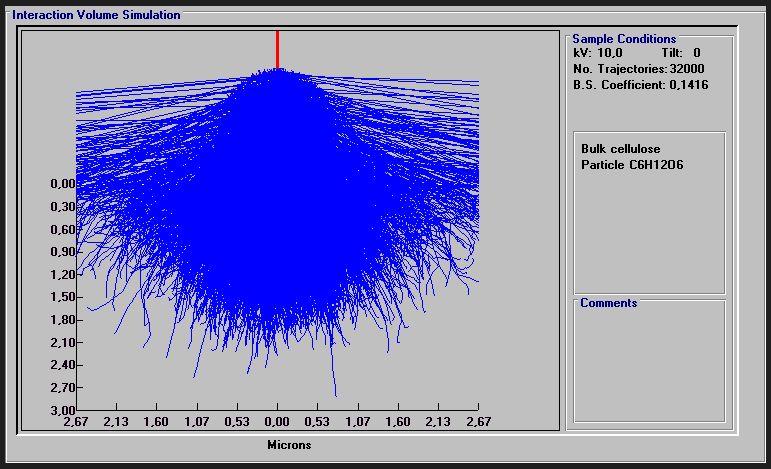
\includegraphics[width =0.5\textwidth]{./figures/simulation10kv.png}
	\end{center}
	\caption{Erzeugte Simulation bei einer Beschleunigungsspannung von \SI{10}{\kilo\volt} \cite{sein_foto}}
    \label{fig:simulation10kv}
\end{figure}


\begin{figure}[H]
	\begin{center}
		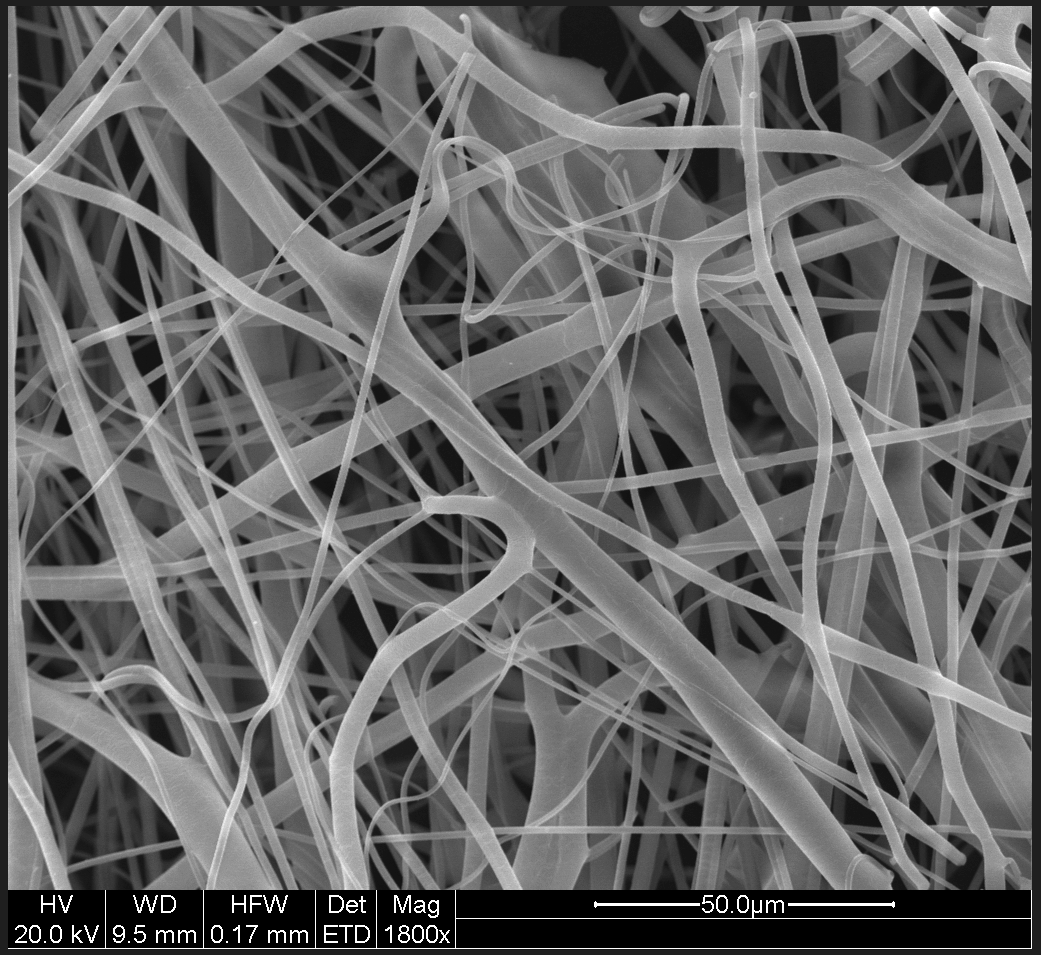
\includegraphics[width =0.5\textwidth]{./figures/20kv.png}
	\end{center}
	\caption{Sichtbares Bild bei einer Beschleunigungsspannung von \SI{20}{\kilo\volt}}
    \label{fig:20kv}
\end{figure}

\begin{figure}[H]
	\begin{center}
		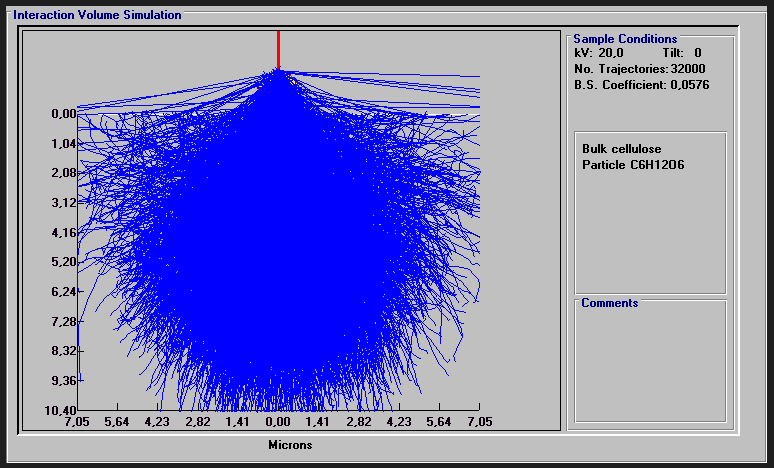
\includegraphics[width =0.5\textwidth]{./figures/simulation20kv.png}
	\end{center}
	\caption{Erzeugte Simulation bei einer Beschleunigungsspannung von \SI{20}{\kilo\volt} \cite{sein_foto}}
    \label{fig:simulation20kv}
\end{figure}



\begin{figure}[H]
	\begin{center}
		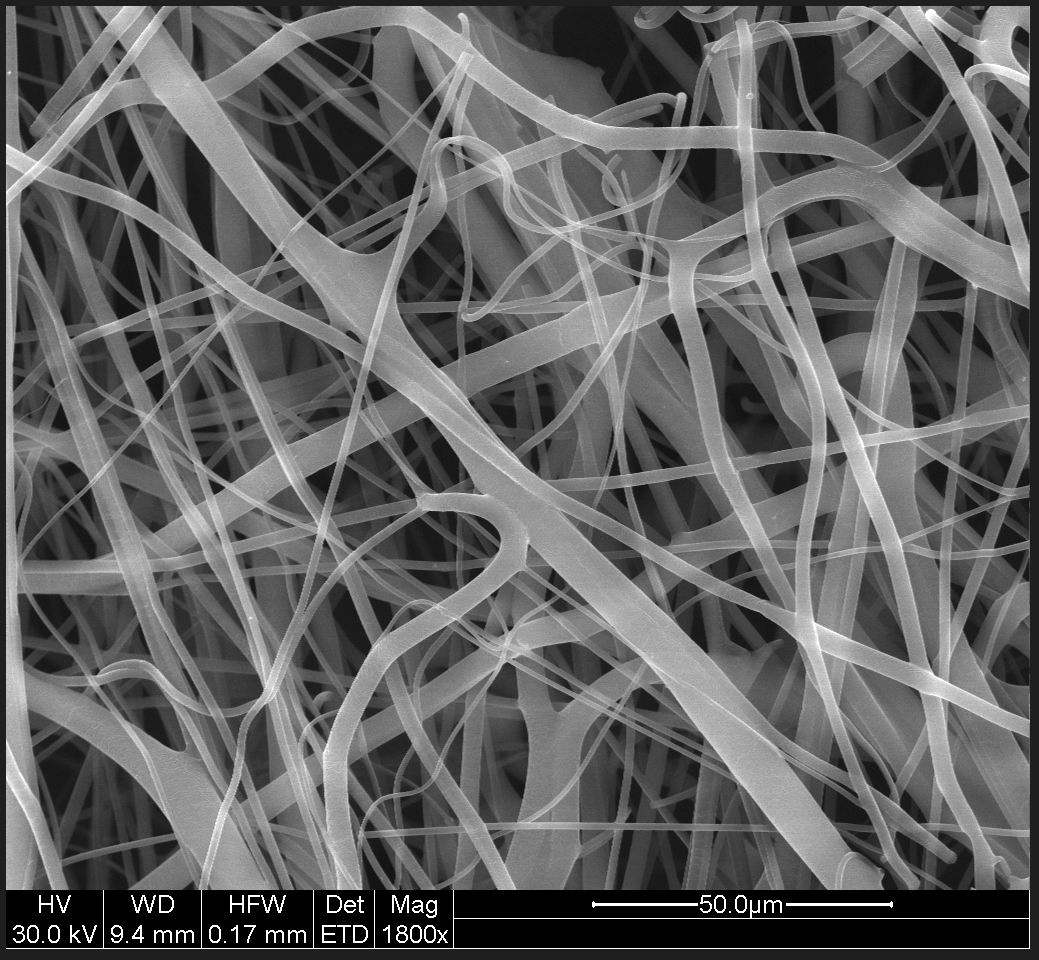
\includegraphics[width =0.5\textwidth]{./figures/30kv.png}
	\end{center}
	\caption{Sichtbares Bild bei einer Beschleunigungsspannung von \SI{30}{\kilo\volt}}
    \label{fig:30kv}
\end{figure}

\begin{figure}[H]
	\begin{center}
		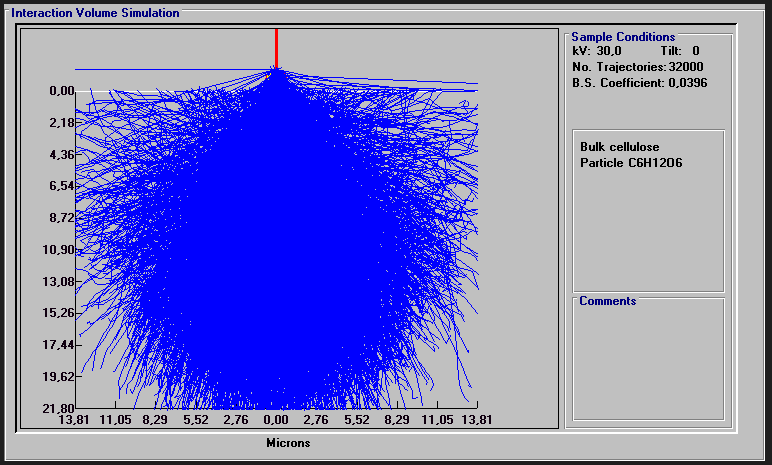
\includegraphics[width =0.5\textwidth]{./figures/simulation30kv.png}
	\end{center}
	\caption{Erzeugte Simulation bei einer Beschleunigungsspannung von \SI{30}{\kilo\volt} \cite{sein_foto}}
    \label{fig:simulation30kv}
\end{figure}

In den erzeugten Fotos ist klar erkennbar, dass bei den kleinen Spannungen besonders die Oberfläche und damit die 
Topografie detektiert wird. Wird die Spannung erhöht werden diese Feinheiten immer undeutlicher und das Bild ähnelt 
immer mehr einer Röntgenaufnahme. Auch an den Simulationen ist klar ersichtlich, dass bei der niedrigen Spannung viele
Elektronen an der Oberfläche gestreut werden und die Anderen in die Probe eindringen. Bei der höheren Beschleunigungsspannung
durchdringen diese jedoch das Gewebe, wodurch die erkennbaren Effekte zu Stande kommen. Die SE, die großteils für die 
Untersuchung der Oberflächentopografie genutzt werden, spielen bei diesem Teil also nicht so eine große Rolle, wie die
BSE und die Röntgenquanten.

\section{Keramik}

Nun wird eine Keramikprobe in den Versuchsaufbau gegeben.

\subsection{Vergleich SE- und BSE-Abbildung}
Bei der Keramikprobe wird nun die gleiche Position jeweils an der gleichen Stelle nur unter Betrachtung der SE oder der BSE
untersucht. 2 so erzeugte Bilder sind nun beispielhaft in \autoref{fig:se} und \autoref{fig:bse} sichtbar.

%todo bitte nebeieinander

\begin{figure}[H]
	\begin{center}
		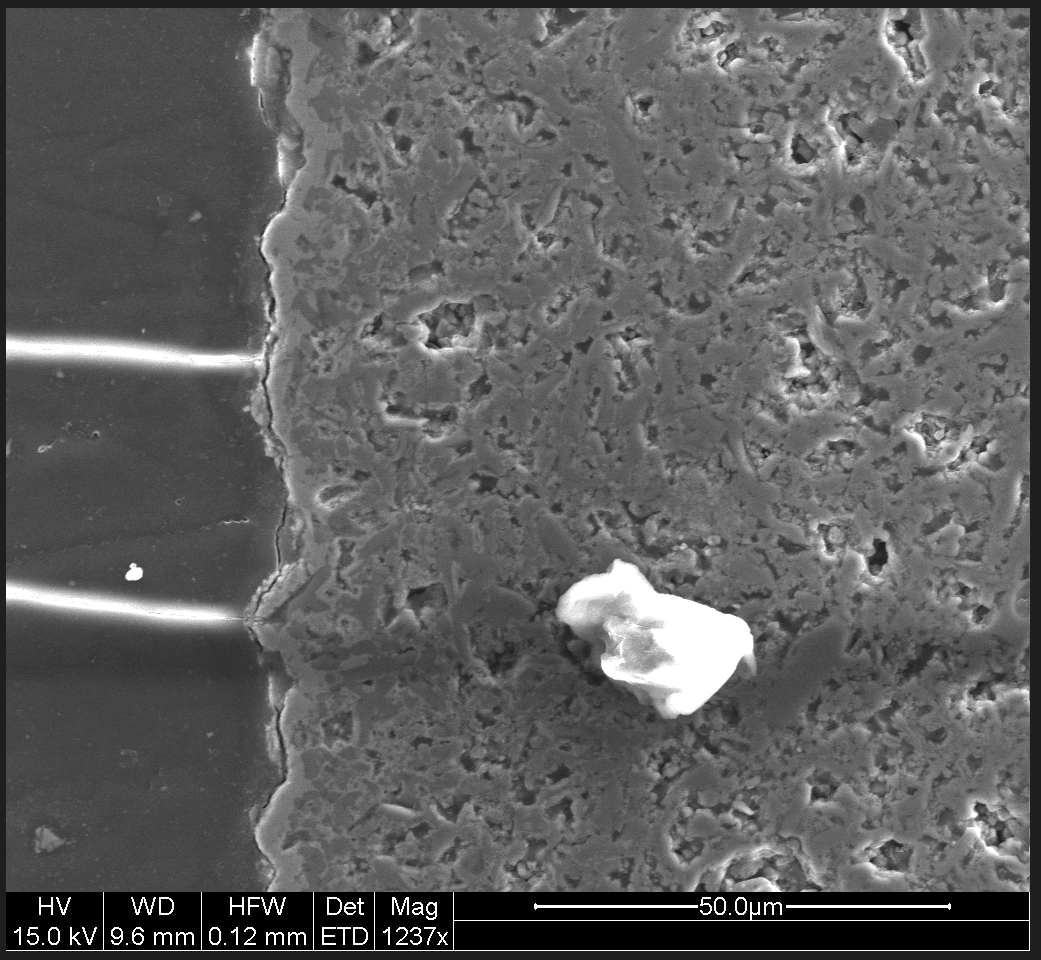
\includegraphics[width =0.5\textwidth]{./figures/se.png}
	\end{center}
	\caption{Erzeugtes Bild mit SE an einer Keramikprobe}
    \label{fig:se}
\end{figure}

\begin{figure}[H]
	\begin{center}
		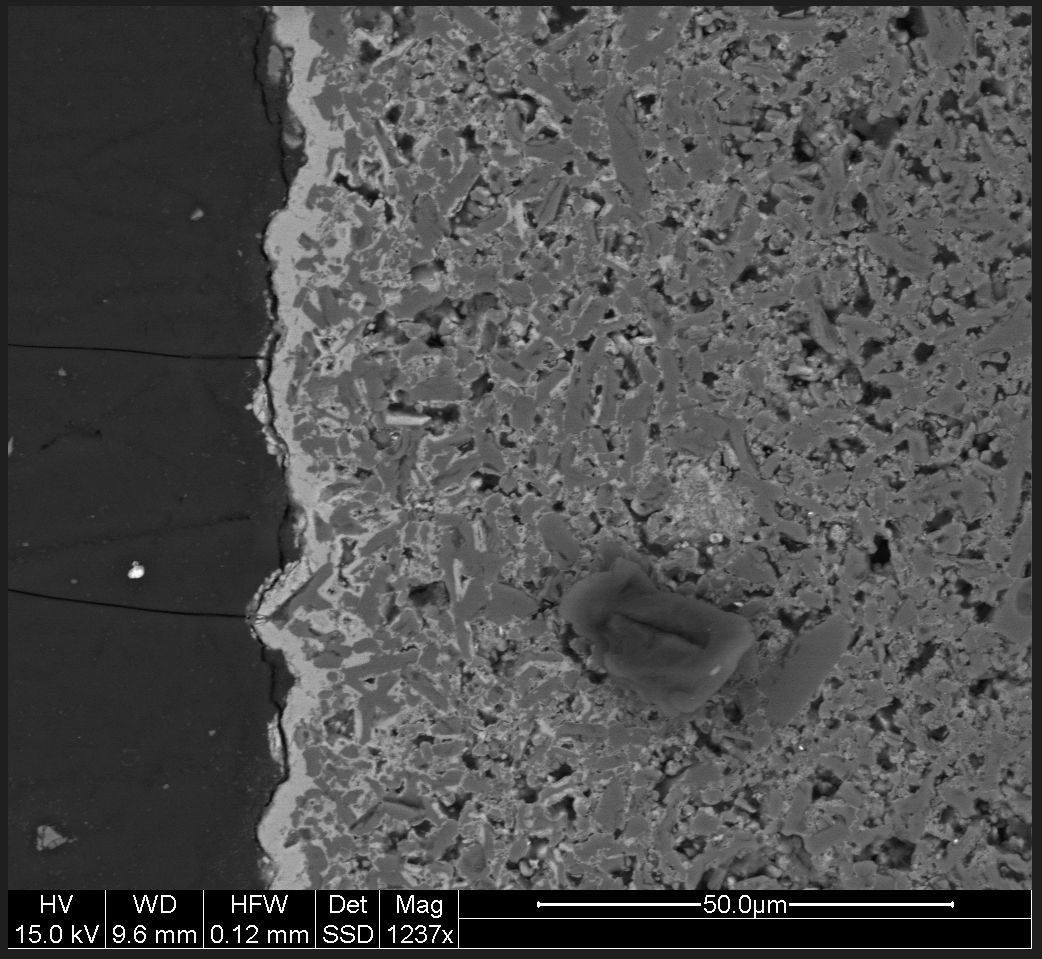
\includegraphics[width =0.5\textwidth]{./figures/bse.png}
	\end{center}
	\caption{Gleiches Bild mit BSE an der Keramikprobe}
    \label{fig:bse}
\end{figure}

Es wird klar ersichtlich, dass bei dem, mit SE erzeugten Bild, insbesondere insbesondere die Oberflächentopografie sichtbar
wird, was besonders an der Erhöhung in der Mitte des Bild erkannt werden kann. Der Grund hierfür ist, dass diese Elektronen
weniger Energie haben und daher nicht so weit in die Probe eindringen. Die BSE dringen in die Probe ein und werden von den 
größeren Atomen stärker zurückgestreut, wodurch ein stärkerer Kontrast, der sogenannte Materialkontrast, sichtbar wird.


\subsection{Bestimmung der Schichtdicke}

Um die Schichtdicke der Keramikprobe zu bestimmen, wird am BSE Bild die entsprechende Schicht vermessen. Mithilfe des automatisch
angezeigten Maßstabs, kann nun die tatsächliche Schichtdicke errechnet werden. Da offensichtlich keine homogen verteilte
Dicke vorliegt, wird diese Messung für mehrere Punkte wiederholt, wie in \autoref{fig:schichtdicke} ersichtlich. Dabei wird 
darauf geachtet, immer den Abstand zu bestimmen, der möglichst orthogonal auf den Rand der Probe liegt. Zusätzlich wurde,
wie in \autoref{fig:schichtdicke} ersichtlich, rein der Interesse halber, auch noch die Größe von 2 Poren bestimmt.

\begin{figure}[H]
	\begin{center}
		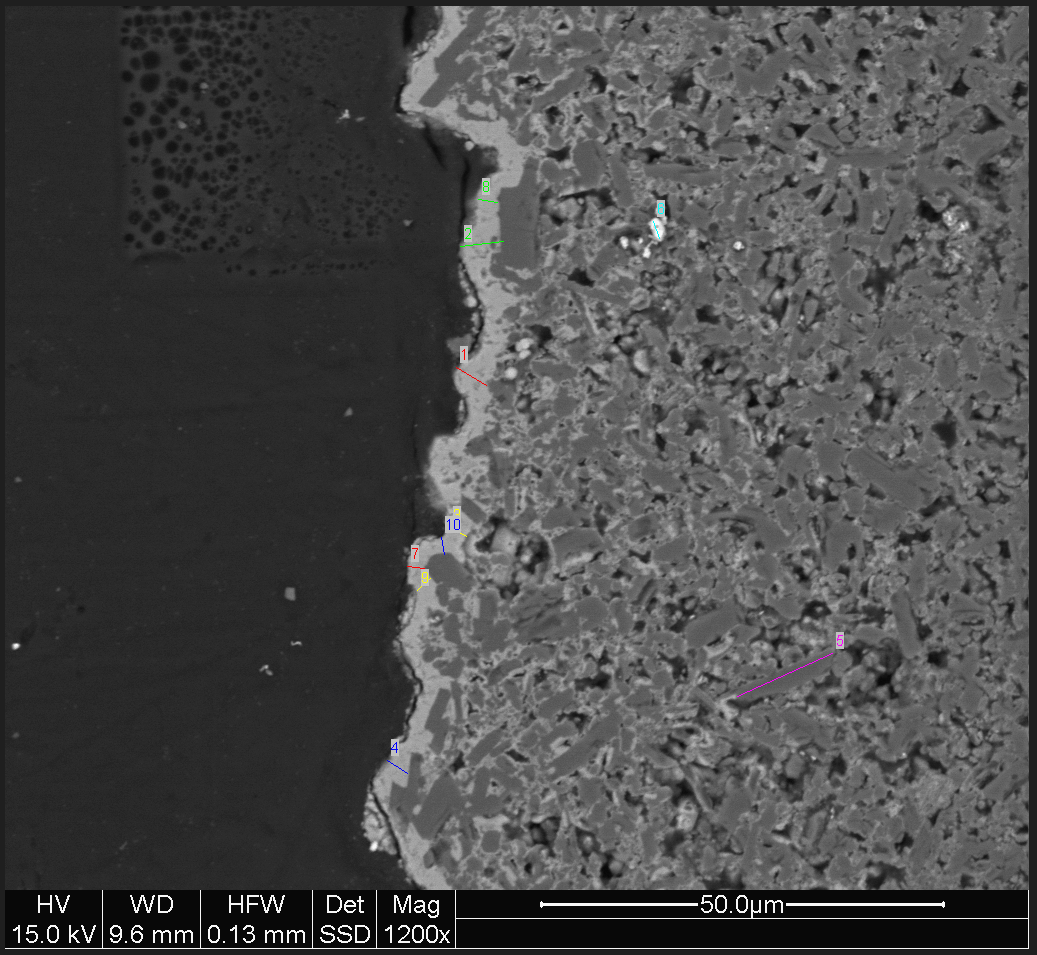
\includegraphics[width =0.8\textwidth]{./figures/schichtdicke.png}
	\end{center}
	\caption{Messung der Schichtdicke auf BSE Bild der Keramikprobe}
    \label{fig:schichtdicke}
\end{figure}

In folgender \autoref{tab:messwerte} sind die erhaltenen Messwerte der Schichtdicke aufgelistet. Die Unsicherheit wurde dabei 
als 1 Pixel angenommen, was im konkreten Fall \SI{100}{\nano\m} entspricht.


\begin{table}[H]
	\caption[Erhaltene Messwerte für die Schichtdicke]{Erhaltene Messwerte für die Schichtdicke\\
	$m_i \dots$ entsprechender Messpunkt\\
	$d \dots$ gemessene Schichtdicke in nm mit einer Unsicherheit von \SI{100}{\nano\m}}
	\begin{center}
	\begin{tabular}{|l|l|}
	\hline
	                 & $d$ / nm         \\ \hline
	$m_{1}$          & \SI{4330}{}      \\ \hline
	$m_{2}$          & \SI{5350}{}      \\ \hline
	$m_{3}$          & \SI{2380}{}      \\ \hline
	$m_{4}$          & \SI{2950}{}      \\ \hline
	$m_{7}$          & \SI{2120}{}      \\ \hline
	$m_{8}$          & \SI{2380}{}      \\ \hline
	$m_{9}$          & \SI{2190}{}      \\ \hline
	$m_{10}$         & \SI{2140}{}      \\ \hline

	\end{tabular}
	\end{center}
	\label{tab:messwerte}
\end{table}

%genau: 2979.14 st 1132

Aus diesen Werten ergibt sich folgende mittlere Schichtdicke $\bar{d}$ mit der Standardabweichung $\sigma$:

\begin{align*}
	\bar{d} = \SI{3000}{\nano\m} \\
	\sigma = \SI{1200}{\nano\m}
\end{align*}

Für die 2 vermessenen Poren ergeben sich folgende Durchmesser:

\begin{align*}
	d_{gross} = \SI{12900(100)}{\nano\m} \\
	d_{klein} = \SI{2230(100)}{\nano\m}
\end{align*}


\section{Qualitative EDX-Analyse}

Unter EDX wird "Energy dispersive x-ray spectroscopy" verstanden. Dies ist eine Analysemethode, um auf die Elemente der 
Probe zu schließen. Dazu wird der Elektronenstrahl auf eine bestimmte Position der Probe gerichtet. Hier werden die
entsprechenden Elektronen in den Atomen ionisiert. "Fallen" nun Elektronen in die so entstandenen Löcher zurück, wird
Energie frei, die in Form von Röntgenquanten ausgestrahlt wird. Anhand dieser Quanten kann nun auf die entsprechenden
Energien und damit auf die Elemente geschlossen werden, da jedem Element ein signifikantes Spektrum zu Grunde liegt.


Dieses vorgehen wurde nun für die Keramikprobe an verschiedenen Positionen wiederholt. Eine höhere Nummer der Position
in \autoref{fig:position1} bis \autoref{fig:position4},
%todo geht die referenz besser?
steht dabei dafür, dass die Analyse weiter innen an der Probe durchgeführt wurde. Auch wurde nur eine Analyse
der Beschichtung, \autoref{fig:beschichtung}, und von reinem Keramik, \autoref{fig:keramik}, durchgeführt. 

\begin{figure}[H]
	\begin{center}
		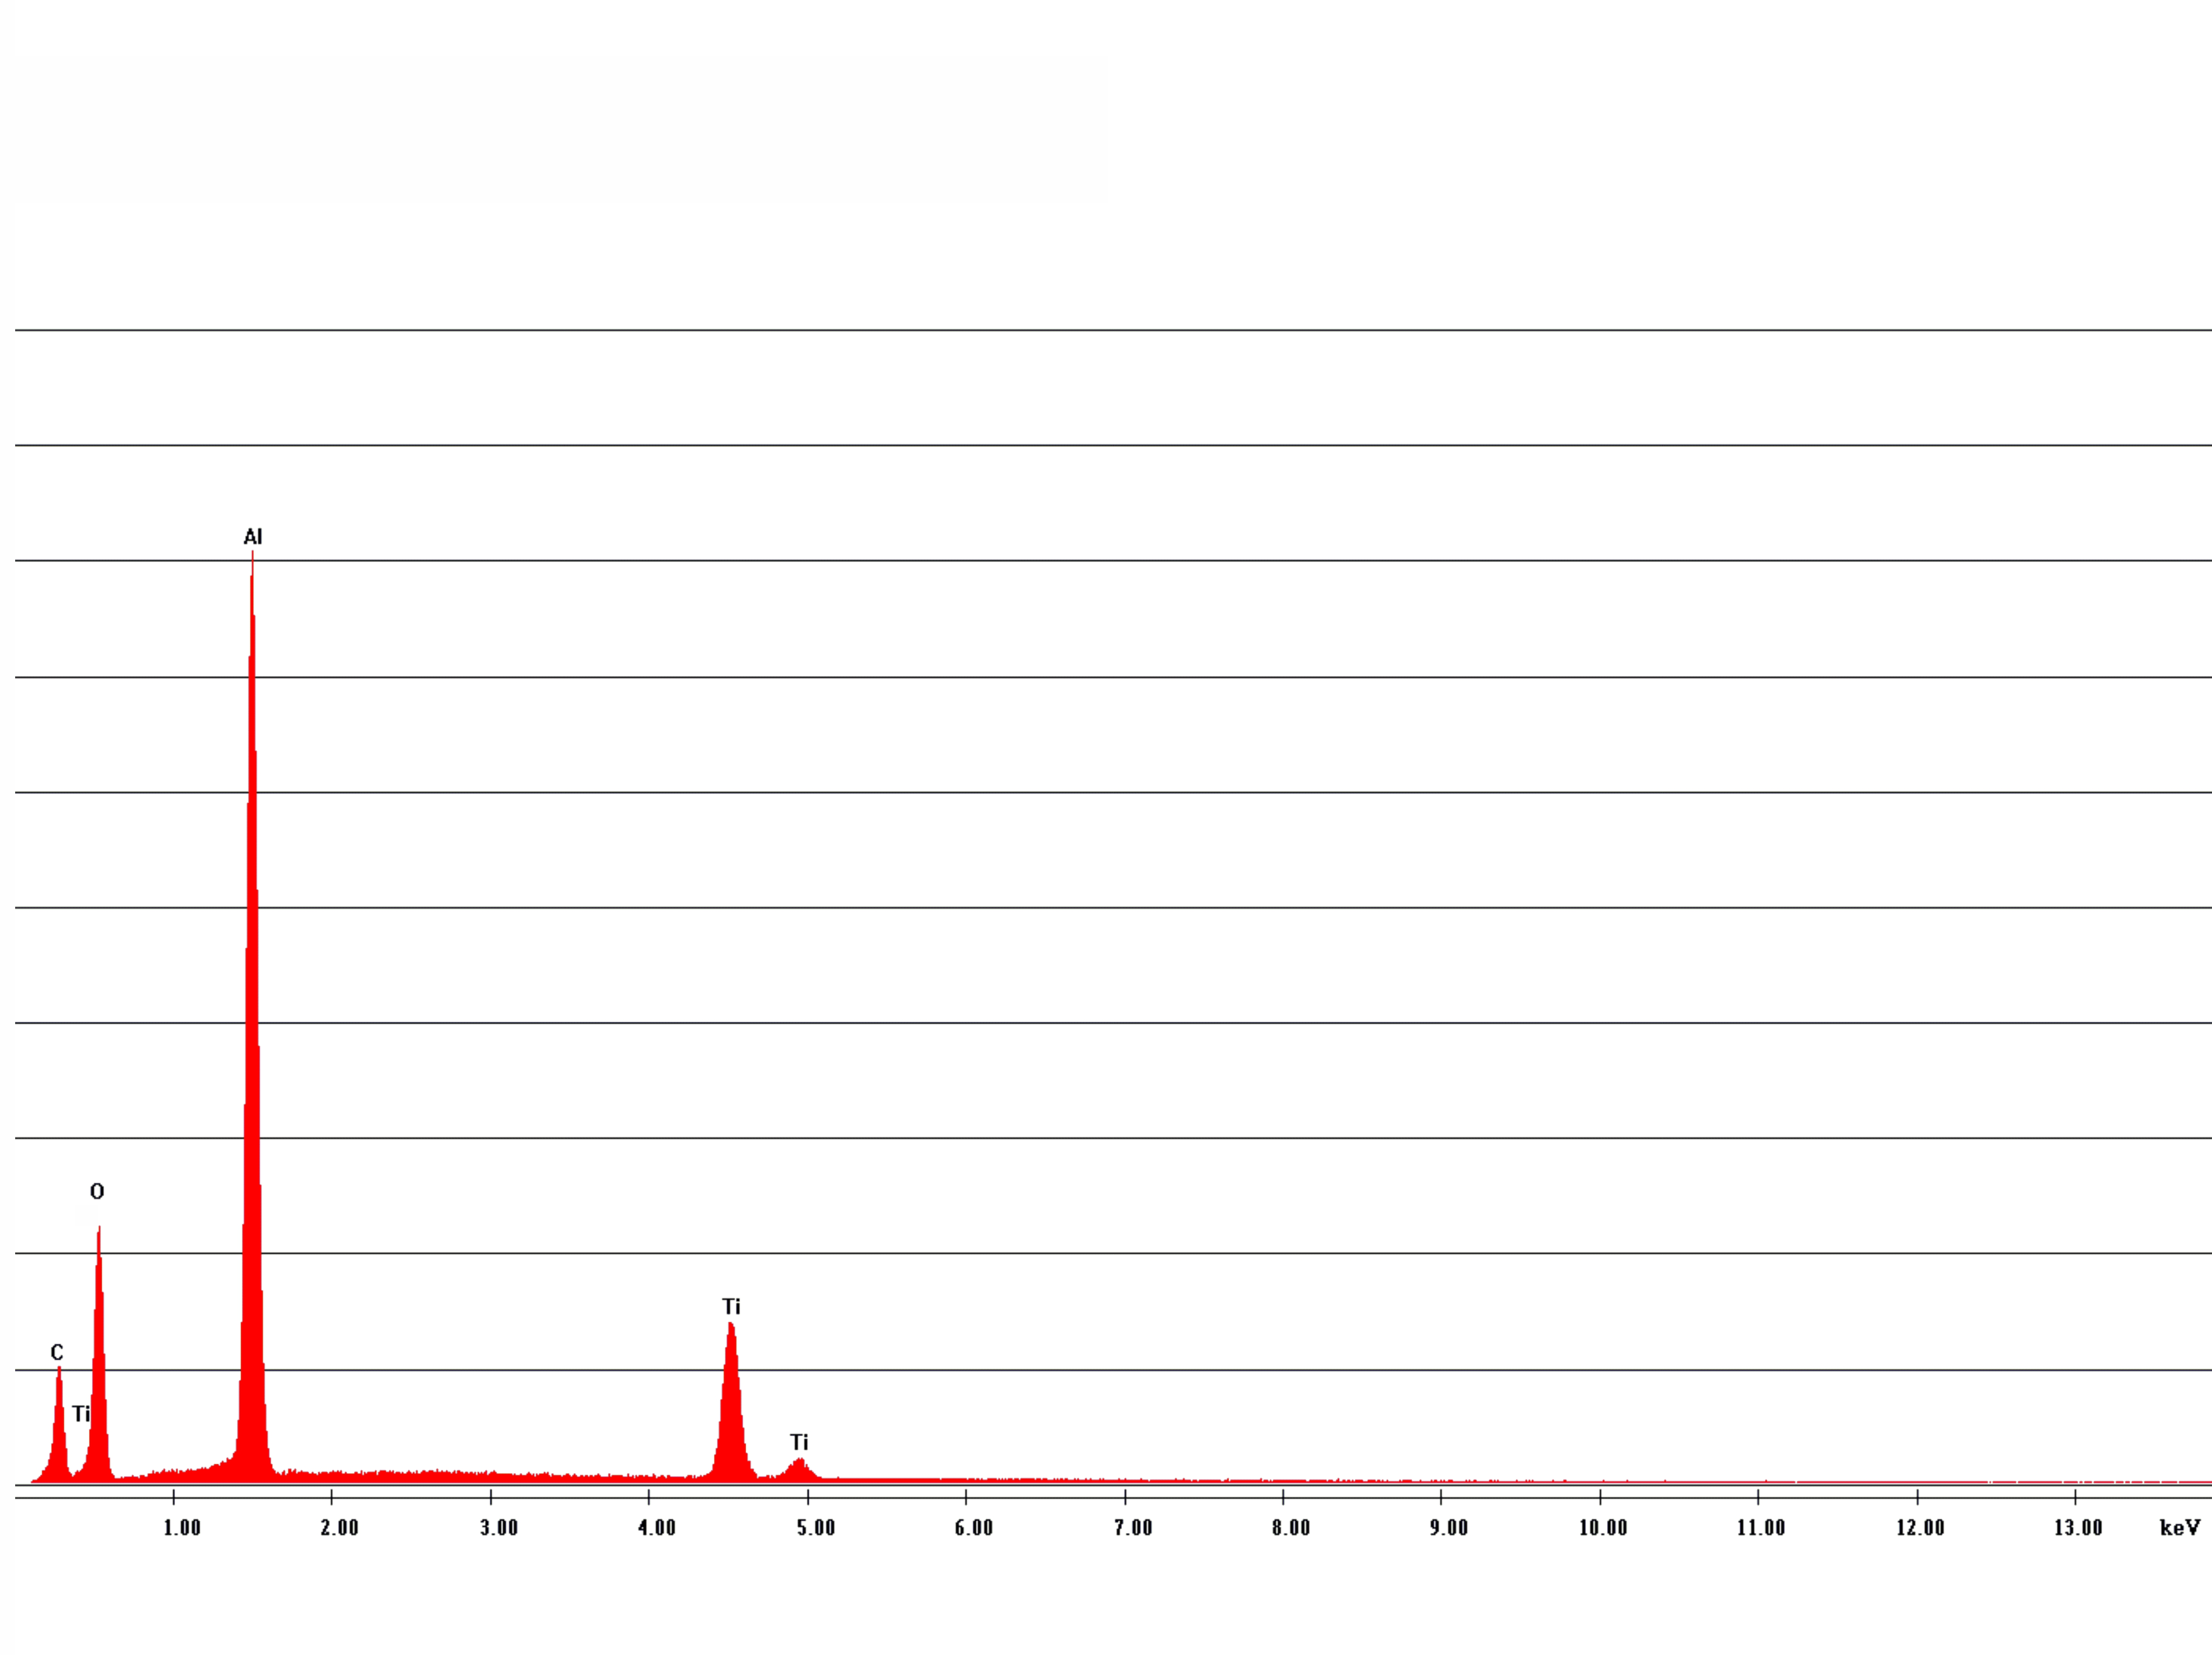
\includegraphics[width =0.8\textwidth]{./figures/edx1.png}
	\end{center}
	\caption{EDX-Analyse der Keramikprobe an Position 1 \cite{sein_foto}}
    \label{fig:position1}
\end{figure}

\begin{figure}[H]
	\begin{center}
		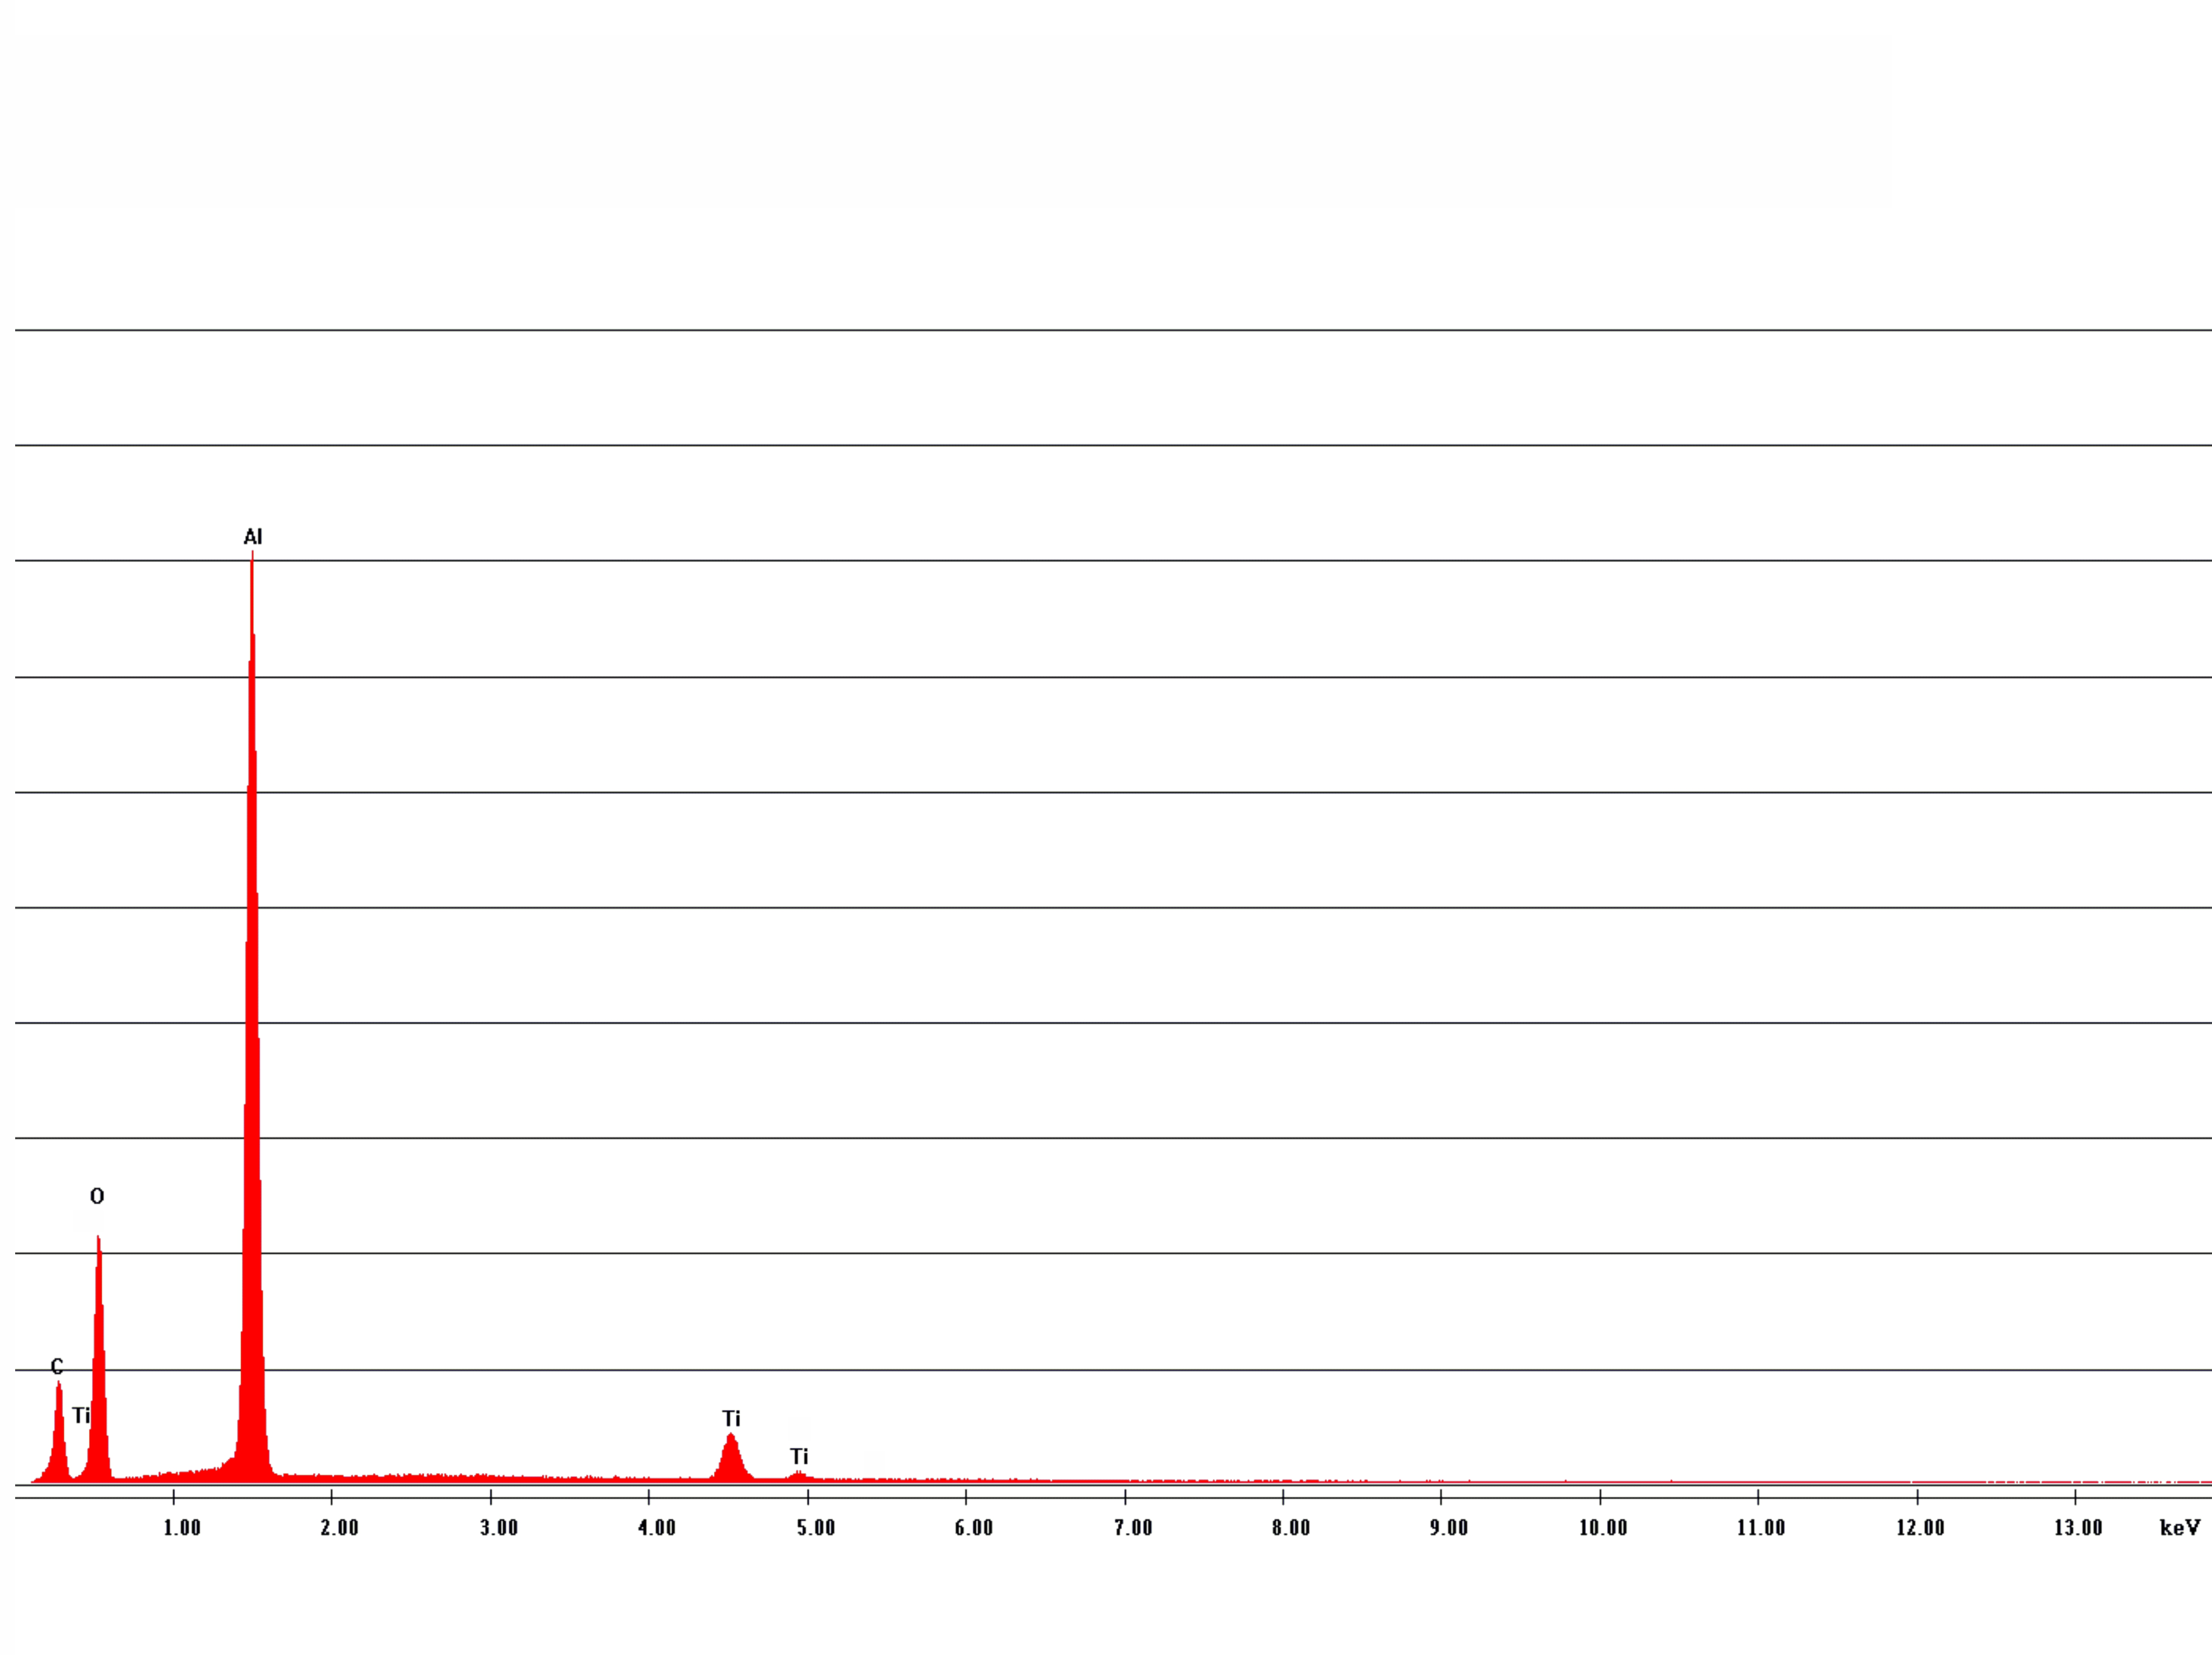
\includegraphics[width =0.8\textwidth]{./figures/edx2.png}
	\end{center}
	\caption{EDX-Analyse der Keramikprobe an Position 2 \cite{sein_foto}}
    \label{fig:position2}
\end{figure}
\begin{figure}[H]
	\begin{center}
		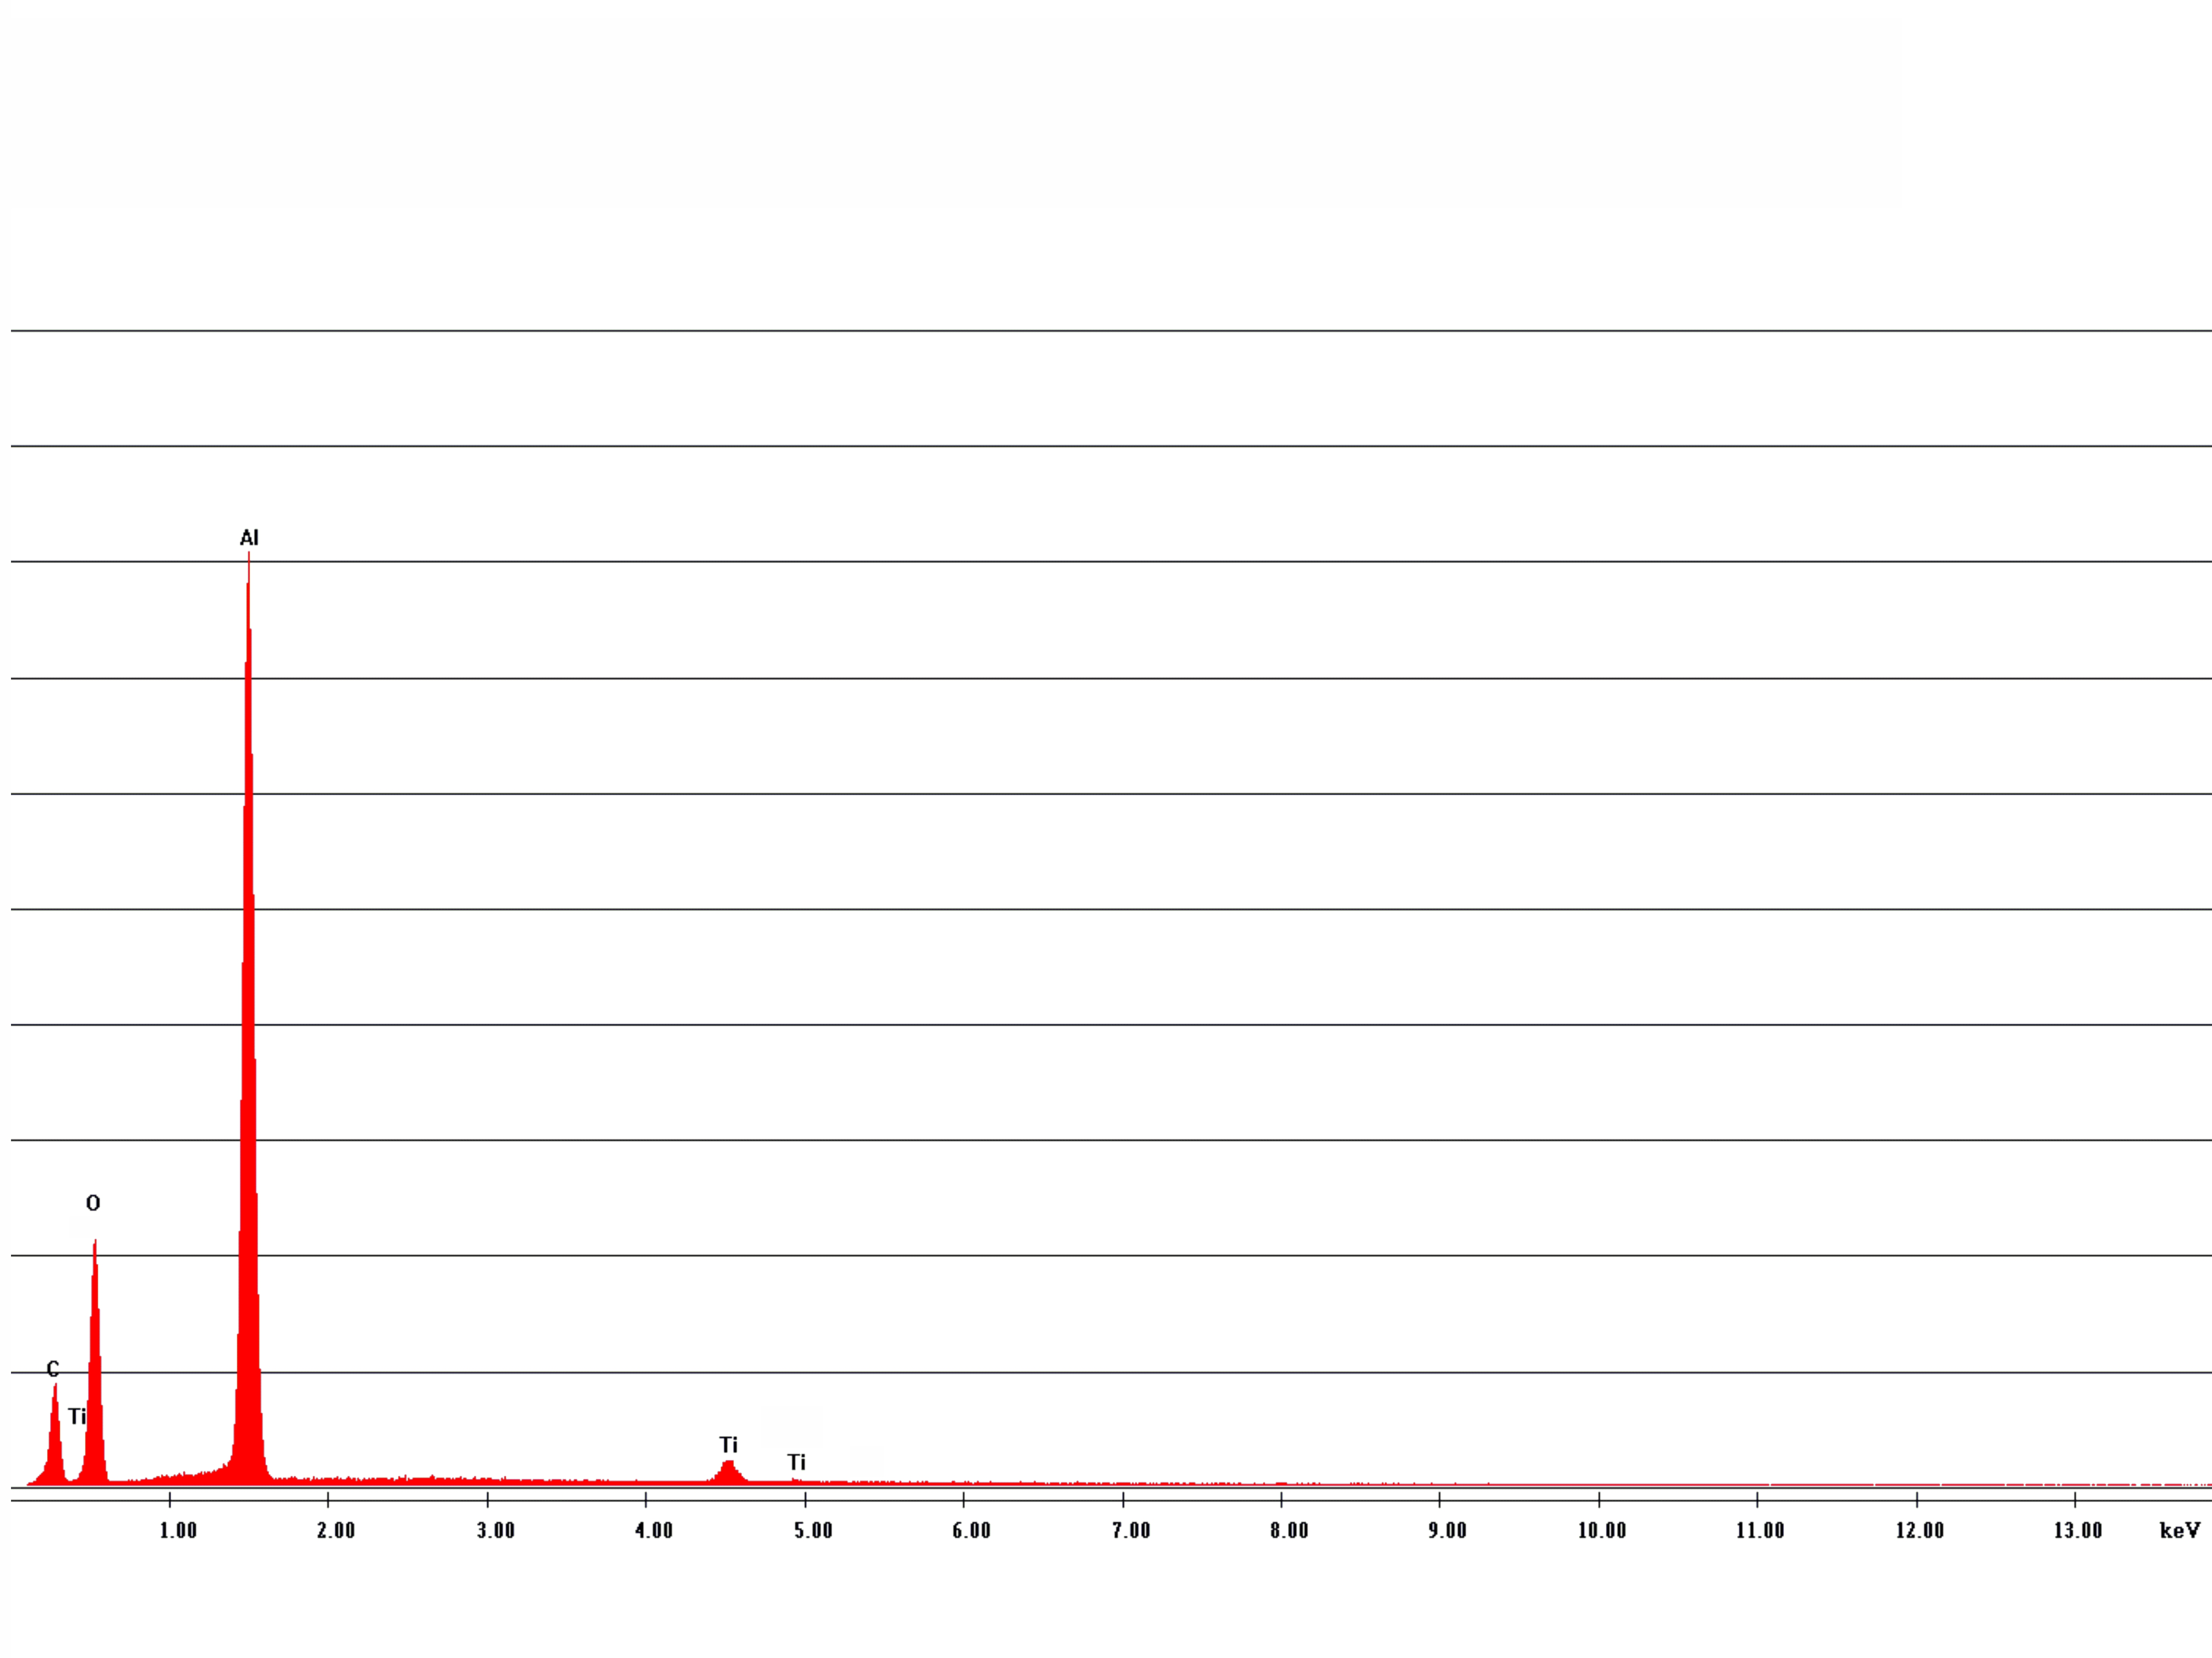
\includegraphics[width =0.8\textwidth]{./figures/edx3.png}
	\end{center}
	\caption{EDX-Analyse der Keramikprobe an Position 3 \cite{sein_foto}}
    \label{fig:position3}
\end{figure}

\begin{figure}[H]
	\begin{center}
		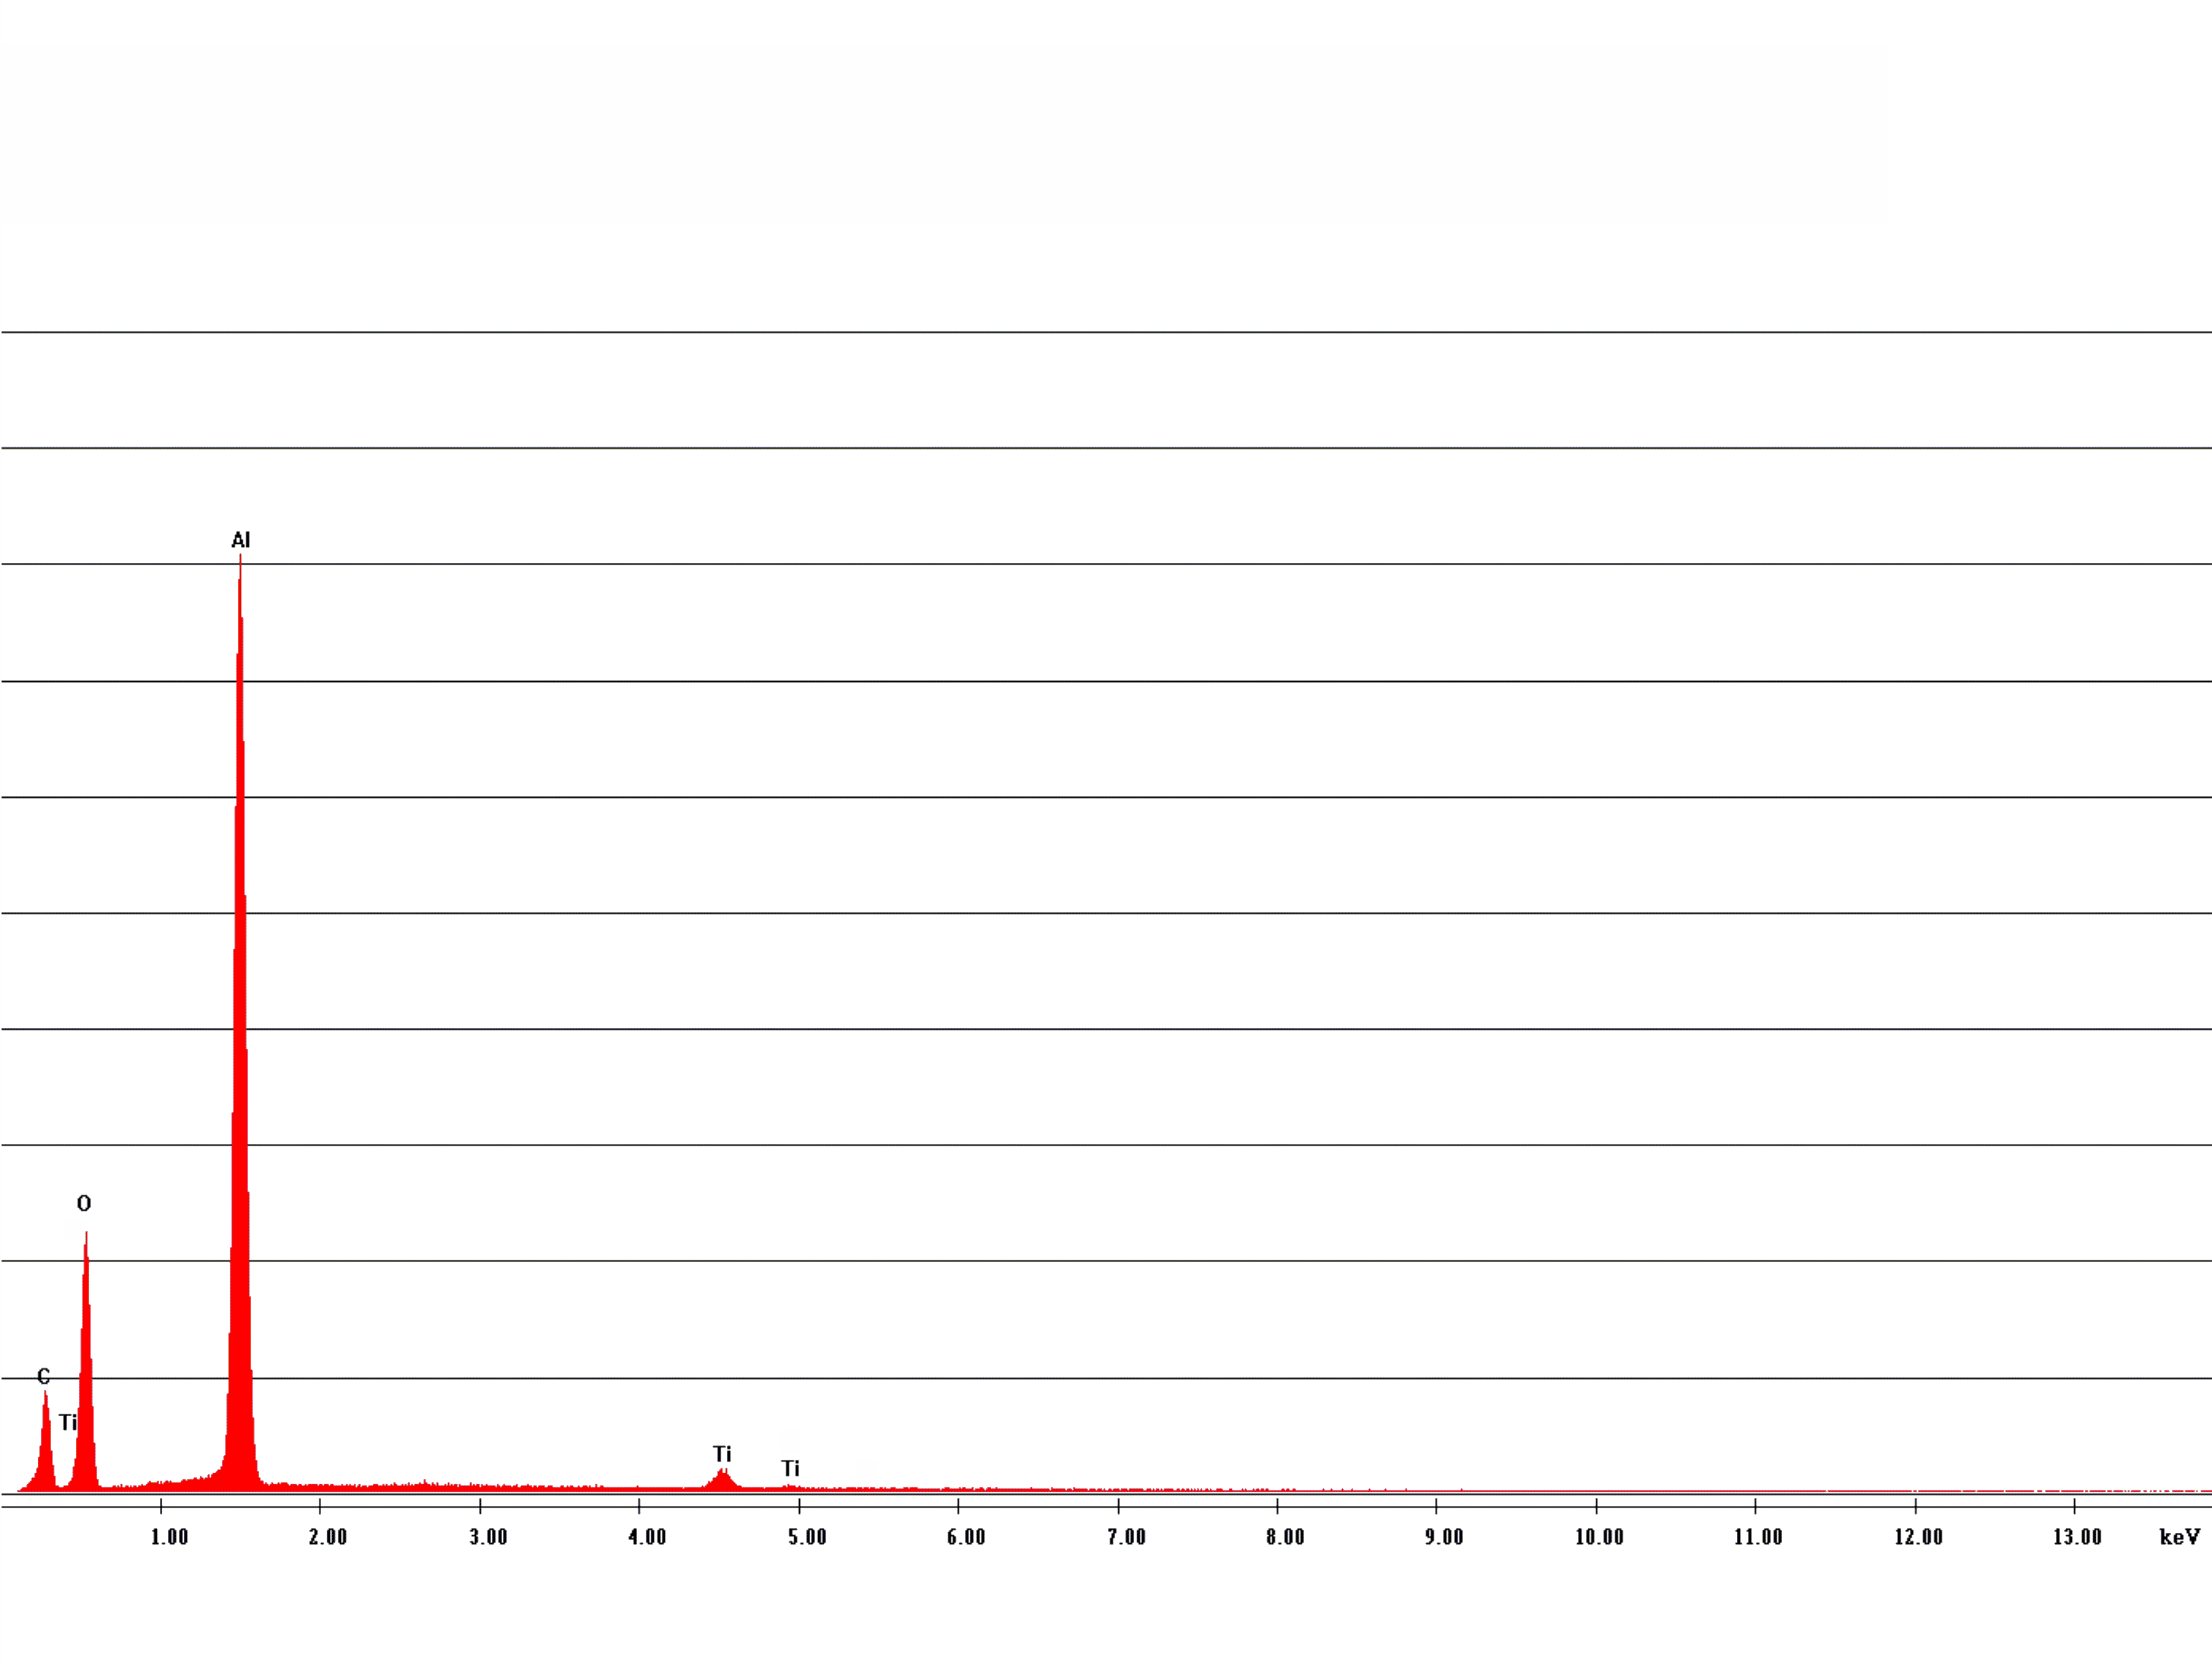
\includegraphics[width =0.8\textwidth]{./figures/edx4.png}
	\end{center}
	\caption{EDX-Analyse der Keramikprobe an Position 4 \cite{sein_foto}}
    \label{fig:position4}
\end{figure}

\begin{figure}[H]
	\begin{center}
		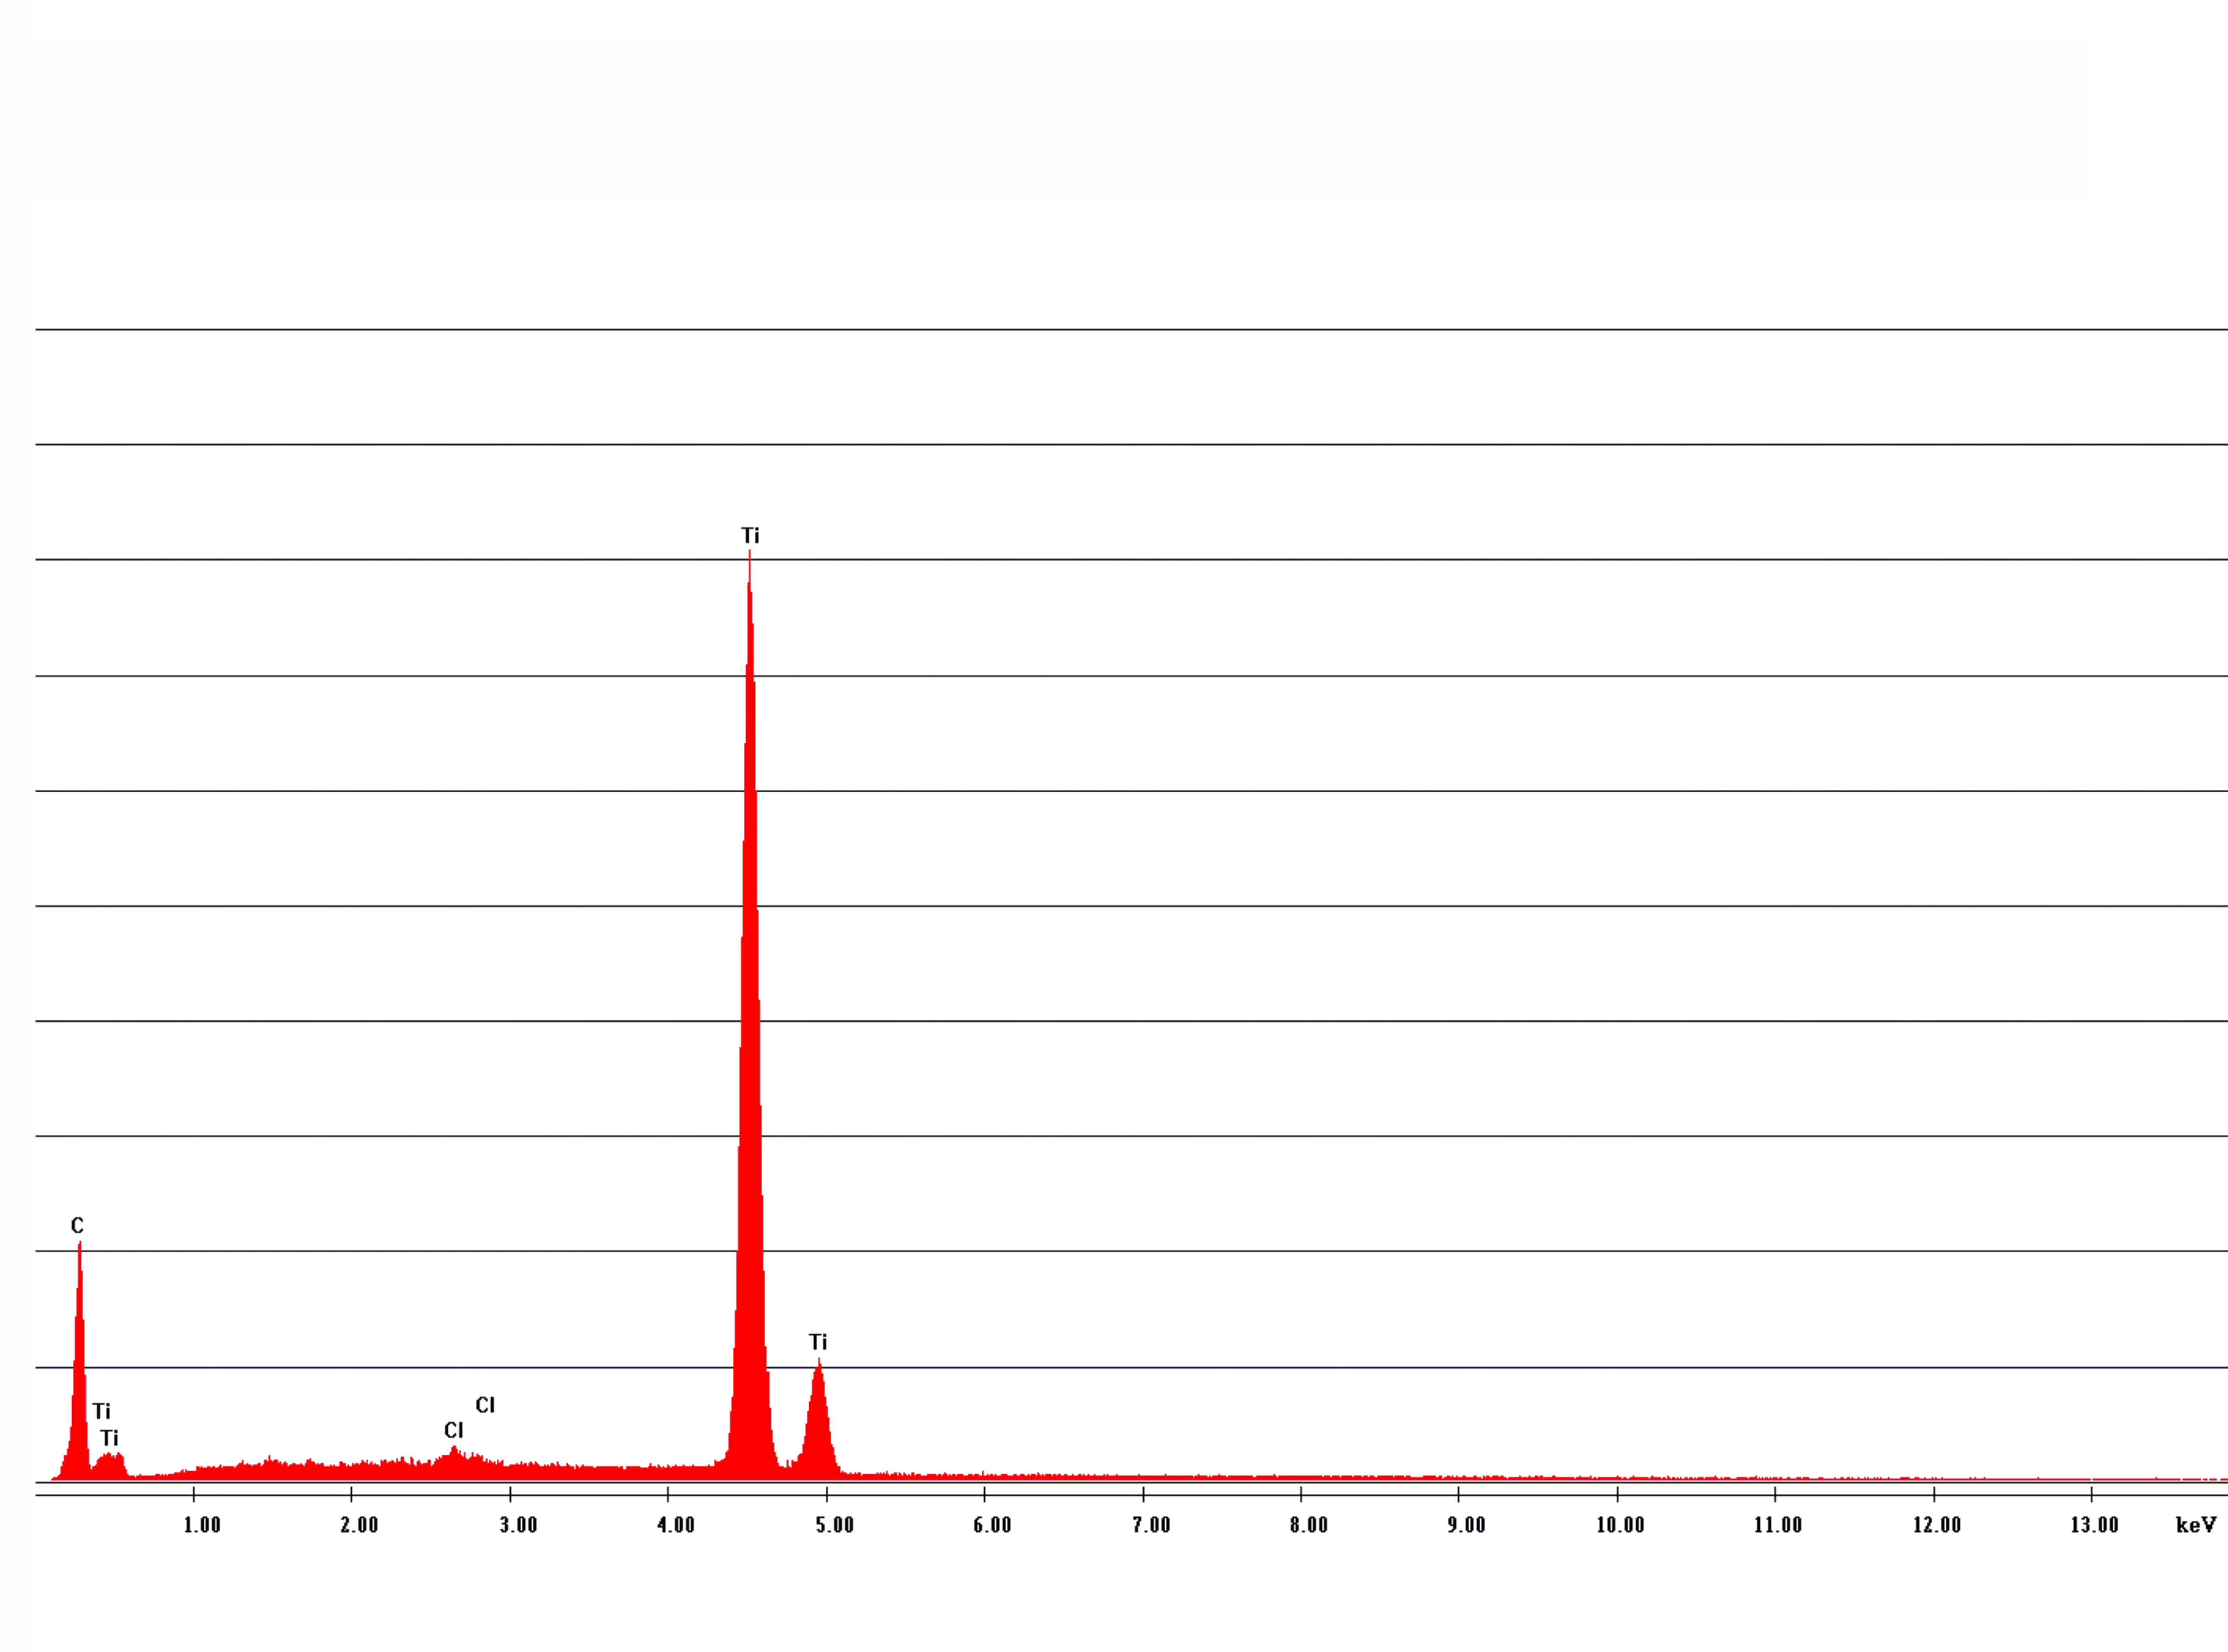
\includegraphics[width =0.8\textwidth]{./figures/beschichtung.png}
	\end{center}
	\caption{EDX-Analyse der Beschichtung \cite{sein_foto}}
    \label{fig:beschichtung}
\end{figure}

\begin{figure}[H]
	\begin{center}
		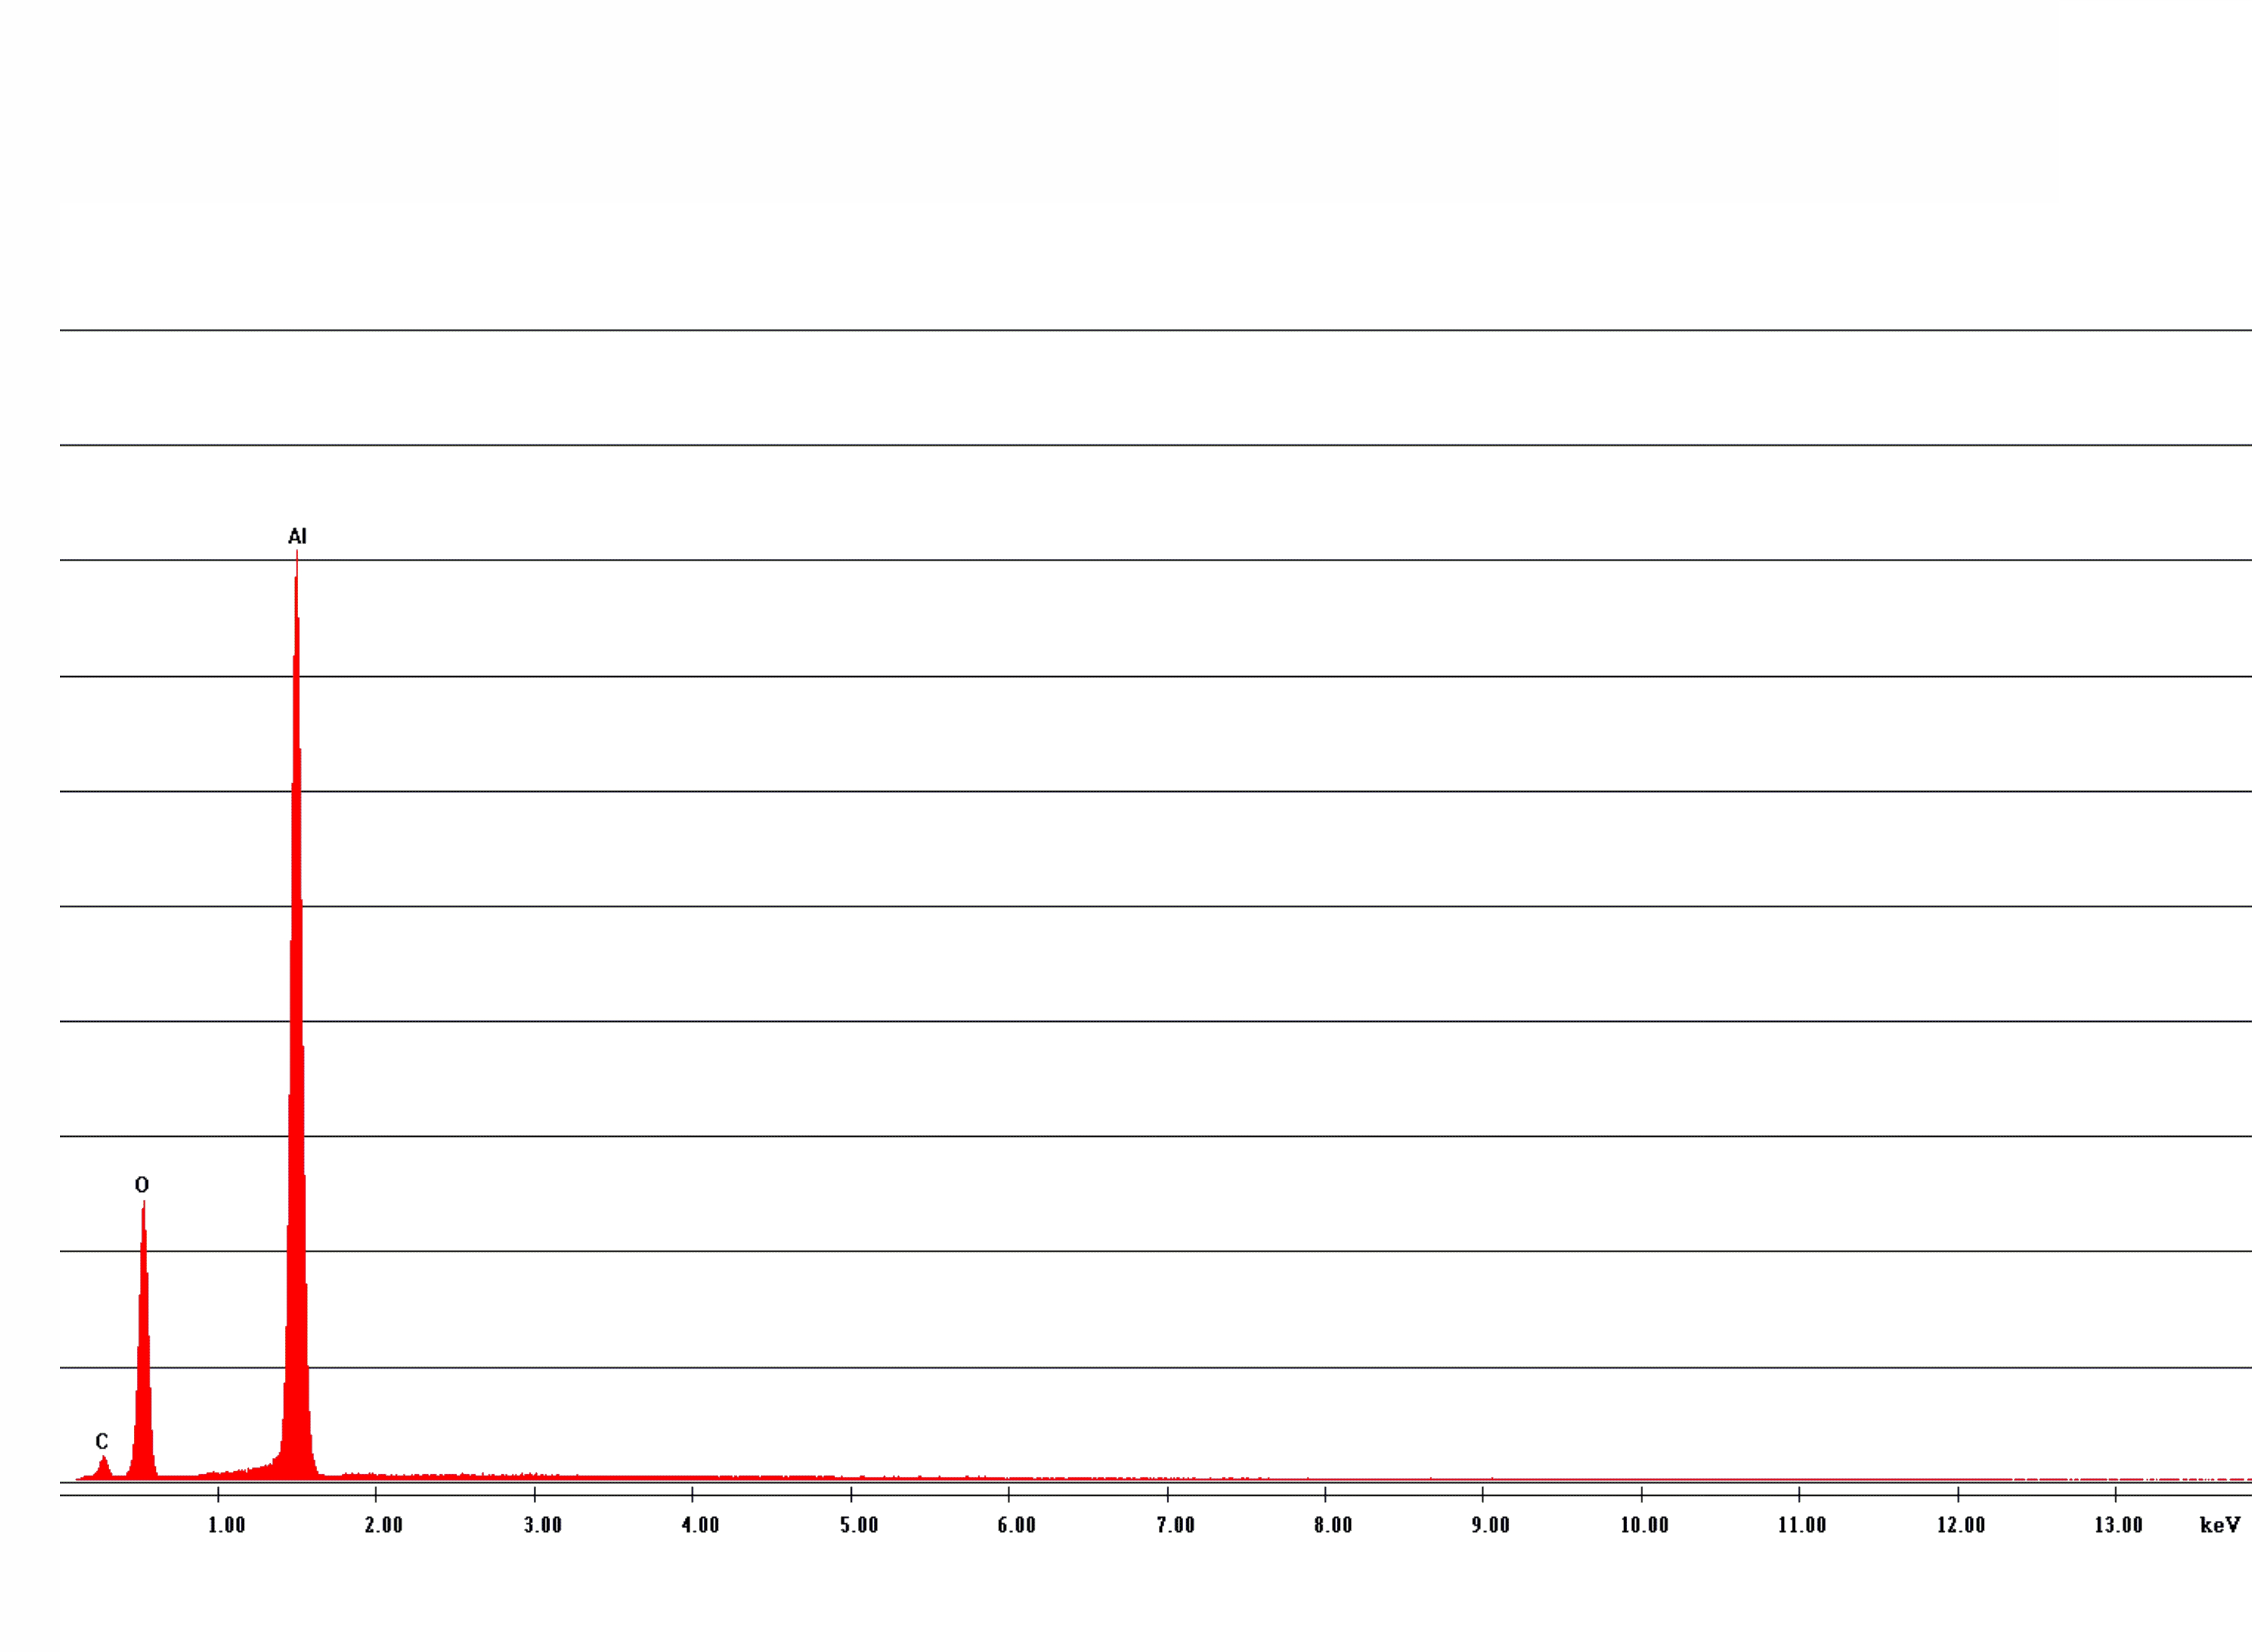
\includegraphics[width =0.8\textwidth]{./figures/keramik.png}
	\end{center}
	\caption{EDX-Analyse der Keramikprobe ohne Beschichtung \cite{sein_foto}}
    \label{fig:keramik}
\end{figure}

Beim Vergleich der einzelnen Positionen wird klar ersichtlich, dass der Ti-Anteil, welcher nach Vergleich mit \autoref{fig:beschichtung}
klar der Beschichtung geschuldet ist, abnimmt, je weiter man sich in das Innere der Probe bewegt. Dies deckt sich auch
mit der Erwartung, da es logisch ist, dass die Beschichtung etwas in die Probe eindringt, der Anteil aber geringer wird, je
weiter man sich vom Rand wegbewegt.


\section{Quantitative EDX-Analyse}


\section{Zusammenfassung}


\section{Anhang}


%Vorbereitungsunterlagen, Daten über Münzen



\newpage

\printbibliography

\end{document}